%%%%%%%% MLSys 2025: LMPool %%%%%%%%%%%%%%%%%

\documentclass{article}

\usepackage{microtype}
\usepackage{graphicx}
\graphicspath{{figures/}}
\usepackage{booktabs}
\usepackage{array}
\usepackage{amsmath}
\usepackage{amssymb}
\usepackage{hyperref}
\urlstyle{same}
\newcommand{\theHalgorithm}{\arabic{algorithm}}

\usepackage[accepted]{mlsys2025}

\makeatletter
\renewcommand{\Notice@String}{}
\def\subsubsection{\@startsection{subsubsection}{3}{\z@}{-0.08in}{0.01in}
                {\normalsize\bf\raggedright}}
\long\def\@makecaption#1#2{%
  \vskip 10pt
  \baselineskip 11pt
  \setbox\@tempboxa\hbox{{\small #1.} #2}%
  \ifdim \wd\@tempboxa >\hsize
    \sbox{\newcaptionbox}{\small #1.~}%
    \newcaptionboxwid=\wd\newcaptionbox
    \usebox\newcaptionbox {\footnotesize #2}%
  \else
    \centerline{{\small #1.} {\small #2}}%
  \fi}
\makeatother

\newcommand{\sys}{LMPool}
\newcolumntype{L}[1]{>{\raggedright\arraybackslash}p{#1}}

\mlsystitlerunning{LMPool: Locality-Aware Routing and NVLink KV-Cache Transfer}

\begin{document}

\twocolumn[
\mlsystitle{LMPool: Locality-Aware Routing and NVLink KV-Cache Transfer for Multi-GPU LLM Serving}

\begin{mlsysauthorlist}
\mlsysauthor{Jialiang Li}{HKUST}
\end{mlsysauthorlist}

\mlsysaffiliation{HKUST}{The Hong Kong University of Science and Technology}
\mlsyscorrespondingauthor{Jialiang Li}{jl.li@connect.ust.hk}

\mlsyskeywords{Large Language Models, KV Cache, Prefix Caching, Multi-GPU Serving, NVLink}

\vskip 0.3in

\begin{abstract}
Prefix caching avoids repeated prefill computation, but independent KV caches in data-parallel LLM replicas can place reusable state on a GPU other than the selected worker, while strict owner routing can overload that worker. This paper presents \sys{}, a multi-GPU LLM serving system that combines KV-aware routing for cache locality with direct NVLink transfer for cache fluidity when placement no longer matches demand. The router balances contiguous ready-prefix reuse against queueing and capacity costs, while a pair- and payload-aware cost model admits copy or move operations only when predicted saved prefill time covers the transfer cost, and a versioned transaction protocol keeps incomplete replicas from routing decisions. On six RTX 3090 GPUs and Qwen3-0.6B and Qwen3-1.7B, 5x shared-prefix routing improves throughput by 11.8\% and 21.3\%, reduces mean TTFT by 18.6\% and 25.2\%, and reduces uncached prefill tokens by 59.9\% and 61.0\% relative to round-robin data parallelism. The packed all-layer K/V microbenchmark validates pair-specific 1-64 block transfer profiles, and the end-to-end results validate background placement and foreground offloading in functionality while showing that completed transfer does not by itself guarantee lower E2E latency or higher throughput. Source code is available at \url{https://github.com/0x0addc001/LMPool}.
\end{abstract}
]
\printAffiliationsAndNotice{}

\section{Introduction}
\label{sec:intro}

PagedAttention~\citep{vLLM} and RadixAttention~\citep{SGLang} make prefix reuse practical within a single inference engine. Multi-GPU deployments, however, typically run one data-parallel model replica and one cache allocator on each GPU. Physical KV blocks remain local to their replicas, whereas requests arrive through a cluster-level ingress. This separation creates a placement problem. An incoming prompt may match a prefix already resident on one GPU, but a conventional round-robin dispatcher may assign the request to another GPU. The selected replica must then recompute and store the same prefix.

A global cache policy can fail in two opposing ways. Routing every matching request to the prefix owner concentrates requests for a hot prefix on one replica, leaves other replicas underutilized, and reduces aggregate batching efficiency. Redistributing KV blocks indiscriminately incurs communication, synchronization, and memory-interference costs even when local recomputation would be cheaper. An effective policy therefore requires the request router and the KV-cache placement mechanism to share a consistent view of locality, load, capacity, and topology.

\sys{} follows two principles. The routing principle addresses cache locality: a request should execute on a GPU that already stores the relevant KV prefix when the reduction in prefill work outweighs the additional queueing and capacity pressure. Effective routing also reduces subsequent data movement. The transfer principle addresses cache fluidity: when KV placement no longer matches request load, direct NVLink transfer can move useful blocks to a replica that can reuse them. Transfer does not resolve arbitrary request skew. Instead, it addresses uneven KV placement and cross-instance reuse that would otherwise require either data movement or recomputation.

The resulting policy prioritizes routing when it can preserve locality and uses the fastest supported direct transfer path only when data movement is both necessary and profitable. \sys{} therefore treats multi-GPU HBM as a logically coordinated pool rather than physically shared memory. Each worker retains ownership of local allocations and KV tensors. The control plane coordinates metadata, reservations, routing decisions, and transfer transactions without accessing the physical KV data.

The design combines a locality- and load-aware router with a cost-gated KV-transfer path. At ingress, the router matches contiguous complete prefix blocks across all healthy replicas and balances saved prefill work against queueing, decode, capacity, and reclamation costs. The transfer path is restricted to direct NVLink pairs, batches complete block chains, supports copy and move semantics, and uses generation checks and rollback within an explicit transaction. This paper makes three contributions. It implements a multi-process system with separate control, allocation, and model-execution ownership. It introduces cost-gated, versioned copy and move transactions coupled with locality- and load-aware routing. It evaluates the data path and three controlled workloads to distinguish stable routing gains, validated transfer mechanisms, and settings in which transfer does not amortize its cost.

\section{Background and Motivation}
\label{sec:bg}

\subsection{Paged KV Caching}

Autoregressive decoding stores key and value vectors for every processed token at every layer. PagedAttention partitions this state into fixed-size physical blocks and maps the logical blocks of each sequence to those physical blocks~\citep{vLLM}. Prefix caching hashes complete logical blocks, which allows two requests with the same hash chain to reference the same ready physical blocks. Block-based allocation reduces fragmentation, while hash-based sharing avoids repeated prefill work. Reuse nevertheless remains limited to the cache allocator that owns the physical block. For a prompt split into complete blocks $b_0,\ldots,b_k$, \sys{} computes a chained hash
\begin{equation}
  h_i = \mathrm{xxhash64}(h_{i-1} \parallel b_i),
\end{equation}
where $h_{-1}$ is empty. Partial tail blocks are not globally reusable. A valid match must start at $h_0$ and remain contiguous, finding an isolated later hash is insufficient because its attention dependencies are absent.

\subsection{Observation 1: Reuse Is a Placement Property}

A prefix-cache hit is useful only when the request executes on a GPU that stores the matching KV state or when transferring that state is cheaper than recomputation. Independent replicas under round-robin placement may retain many local cache entries yet fail to use them at request admission. In contrast, a global router can increase request-level and token-level reuse without increasing physical cache capacity. Routing should therefore be considered before data movement.

\subsection{Observation 2: Locality Competes with Load Balance}

Long shared prefixes often receive many requests. Sending every matching request to the first owner converts cache locality into a load hotspot. Aggregate hit rate alone cannot expose this failure, so the evaluation must include per-rank request counts, token counts, prefill and decode time, GPU utilization, and memory utilization. A routing decision must account for the remaining prefill work, queued tokens, active decode work, free blocks, and reclamation pressure. The objective is not to maximize hit rate, but to minimize expected completion cost.

\subsection{Observation 3: Transfer Must Earn Its Cost}

Direct NVLink is faster than host-mediated storage paths on the evaluated node, but each transfer reserves destination blocks, synchronizes two workers, consumes link and memory bandwidth, and updates control metadata. Short-lived or cold KV state should be recomputed or evicted rather than transferred. Transfer becomes attractive when a complete hot chain is likely to be reused, when a session moves to a different replica, or when preserving reusable state relieves an actual local block shortage. This observation motivates transfer batching, cost estimation based on measured bandwidth, and separate admission policies for foreground and background transfer.

\subsection{Scope}

\sys{} targets replicas of the same model on a multi-GPU node with direct NVLink pairs that are either configured explicitly or discovered automatically. Ingress routing can select any healthy replica because the request has not yet been assigned to a worker. Worker-originated rerouting and every KV-transfer plan are limited to the current GPU and its configured direct NVLink partners, unrelated PCIe or NUMA peers are not used as transfer paths. The system complements RDMA-based and storage-tier systems rather than replacing them. Cross-node RDMA, CPU/SSD tiers, heterogeneous models, and transparent remote memory addressing remain outside the current scope.

\section{System Design}
\label{sec:design}

\begin{figure*}[t]
  \centering
  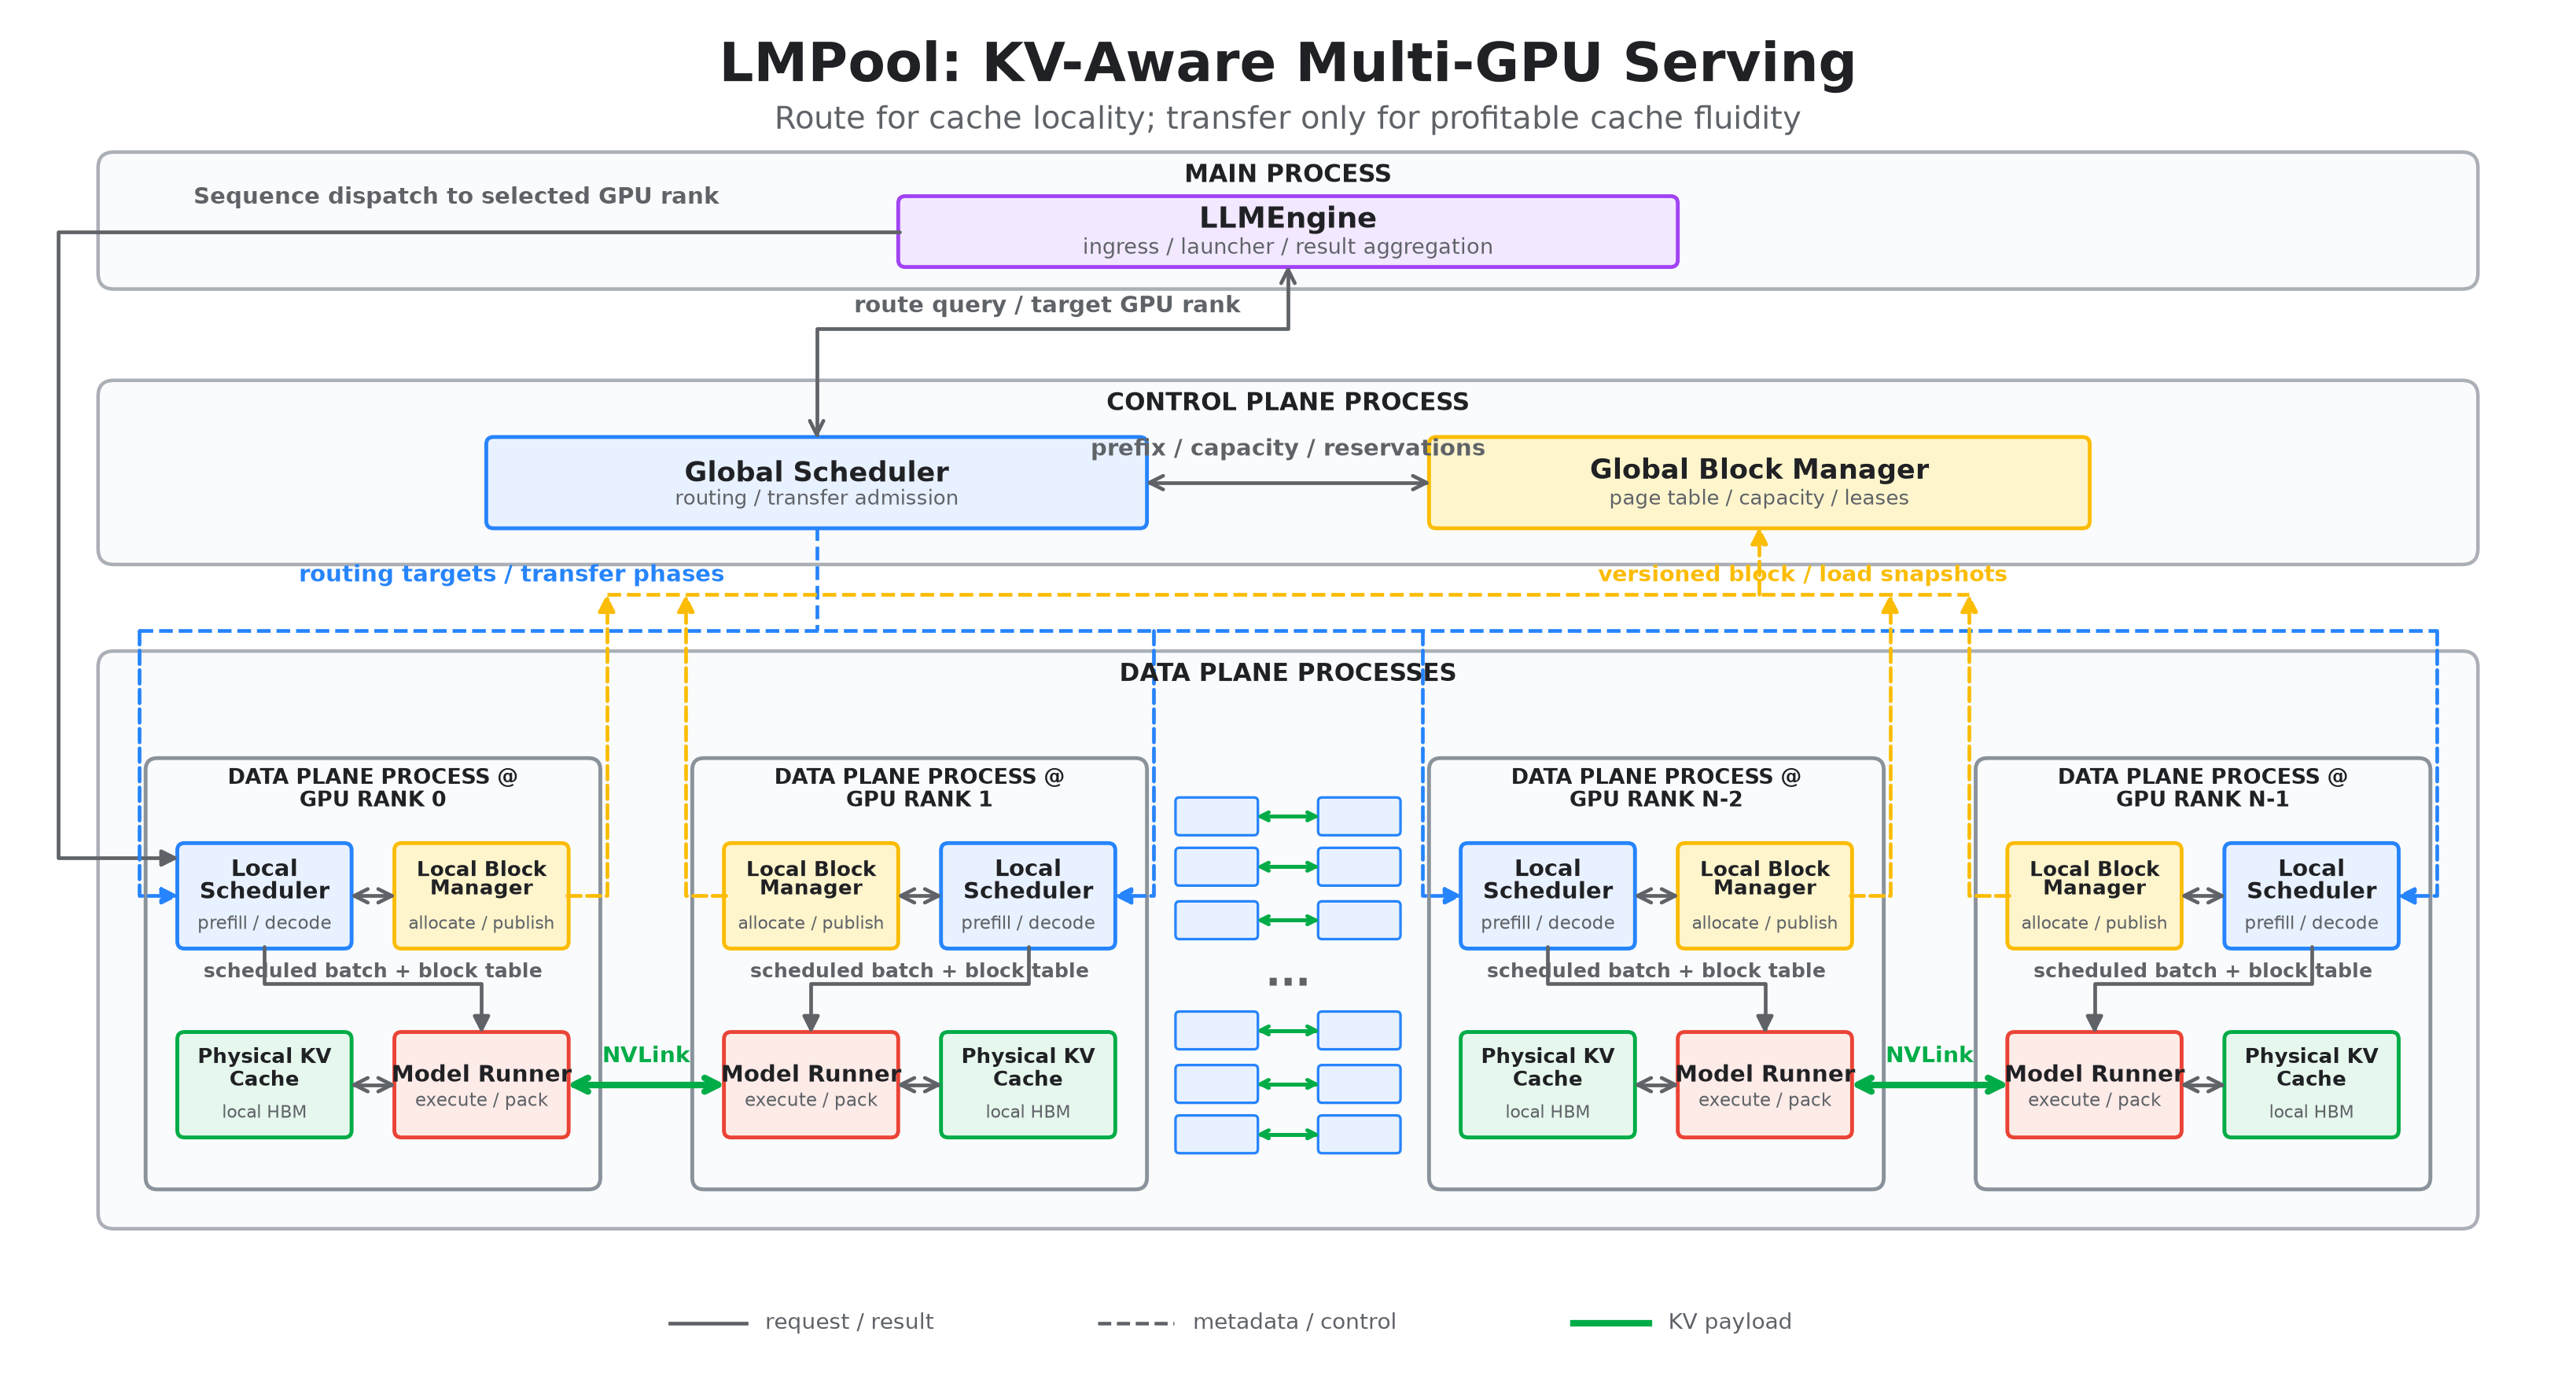
\includegraphics[width=0.92\textwidth]{fig_architecture.png}
  \caption{\sys{} separates request, control, metadata, and KV data paths across the main process, control plane, and per-GPU data planes. Global Scheduler sends routing and transfer commands to every Local Scheduler, while every Local Block Manager publishes versioned block and load snapshots to Global Block Manager. Only paired Model Runners exchange packed KV tensors over the NVLink path, physical KV data never traverses the control plane.}
  \label{fig:arch}
\end{figure*}

Figures~\ref{fig:routing-decision}-\ref{fig:transfer-decision} distinguish three operations that are often conflated. Routing selects the GPU on which a request executes, background placement predicts demand and admits a candidate replica, and transactional transfer validates and executes an admitted plan. The decision nodes show the rejection, deferral, spill, and rollback paths. A hotness threshold cannot bypass the capacity, cooldown, pair-idleness, or measured-cost checks.

\begin{figure*}[t]
  \centering
  
\includegraphics[width=0.9\textwidth]{fig_routing_decision.png}
  \caption{KV-aware routing filters infeasible GPUs and selects a rank according to contiguous-prefix reuse, projected load, and capacity. A bounded spill bypasses the prefix owner only when its load is sufficiently higher and the additional recomputation cost remains limited.}
  \label{fig:routing-decision}
\end{figure*}

\begin{figure*}[t]
  \centering
  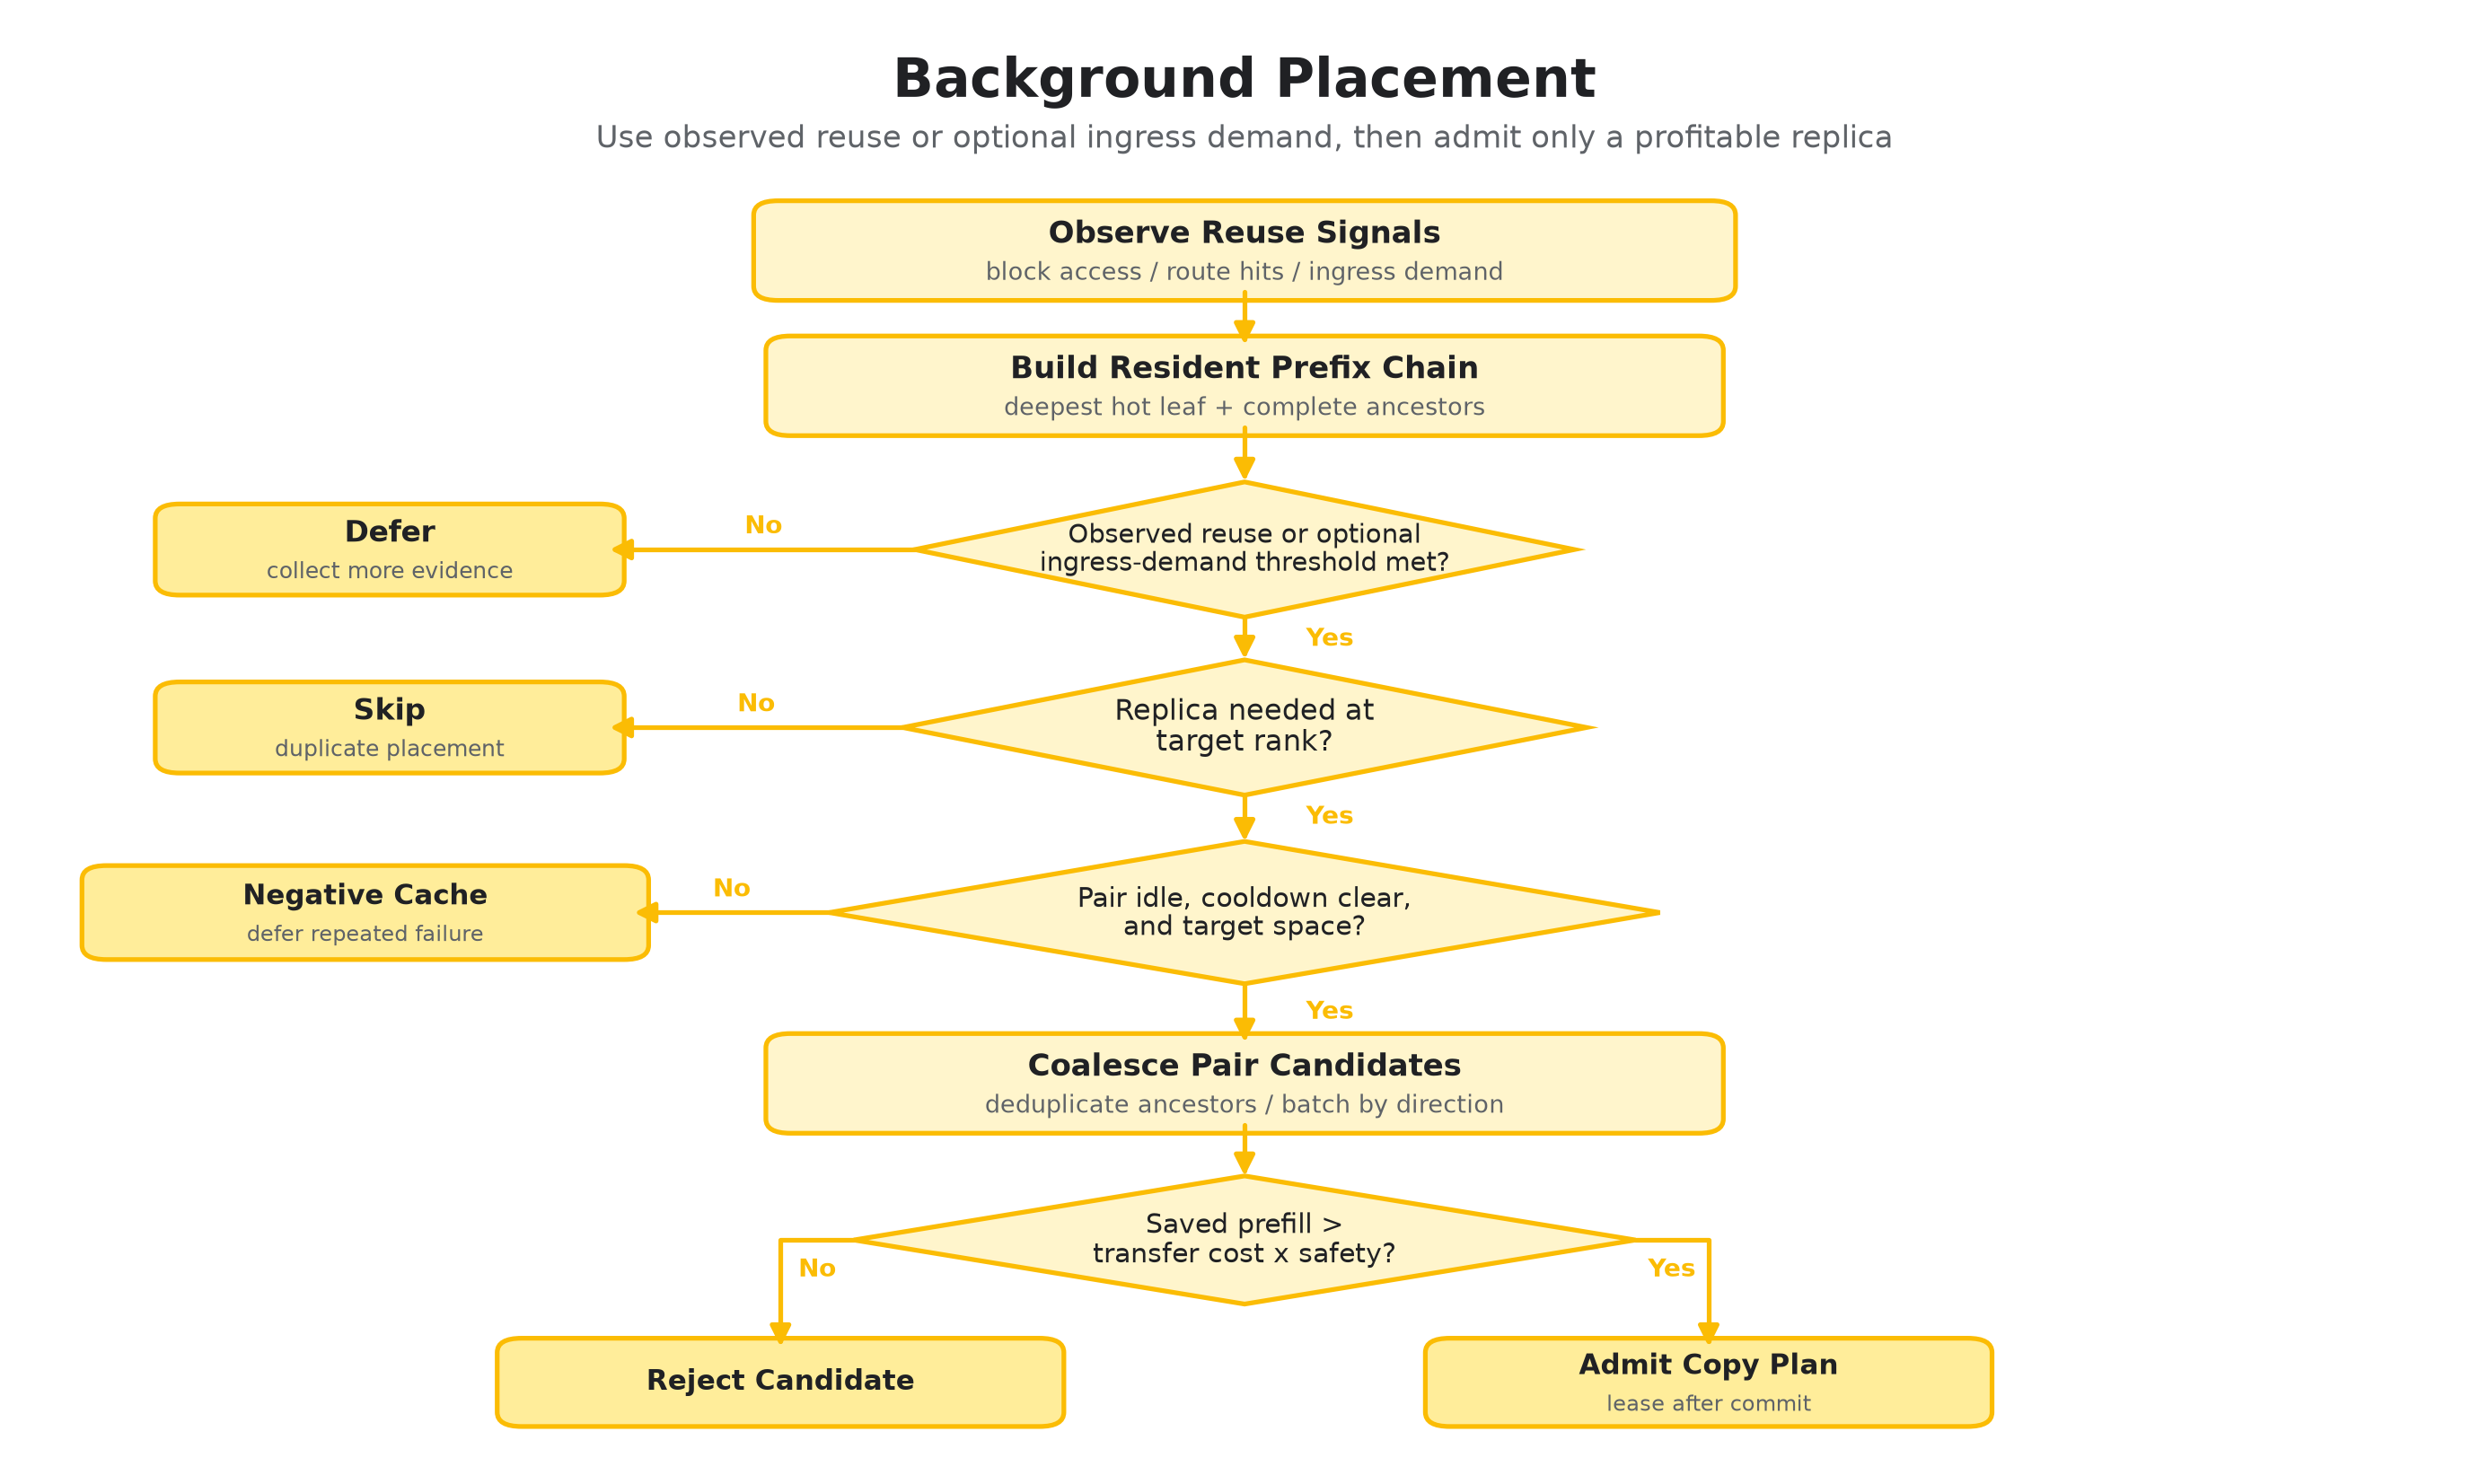
\includegraphics[width=0.9\textwidth]{fig_hot_prefix_decision.png}
  \caption{Background placement admits a candidate replica only when complete-block observations or ingress forecasts indicate demand and the cooldown, pair-idleness, target-capacity, and measured-benefit checks pass.}
  \label{fig:hot-prefix-decision}
\end{figure*}

\begin{figure*}[t]
  \centering
  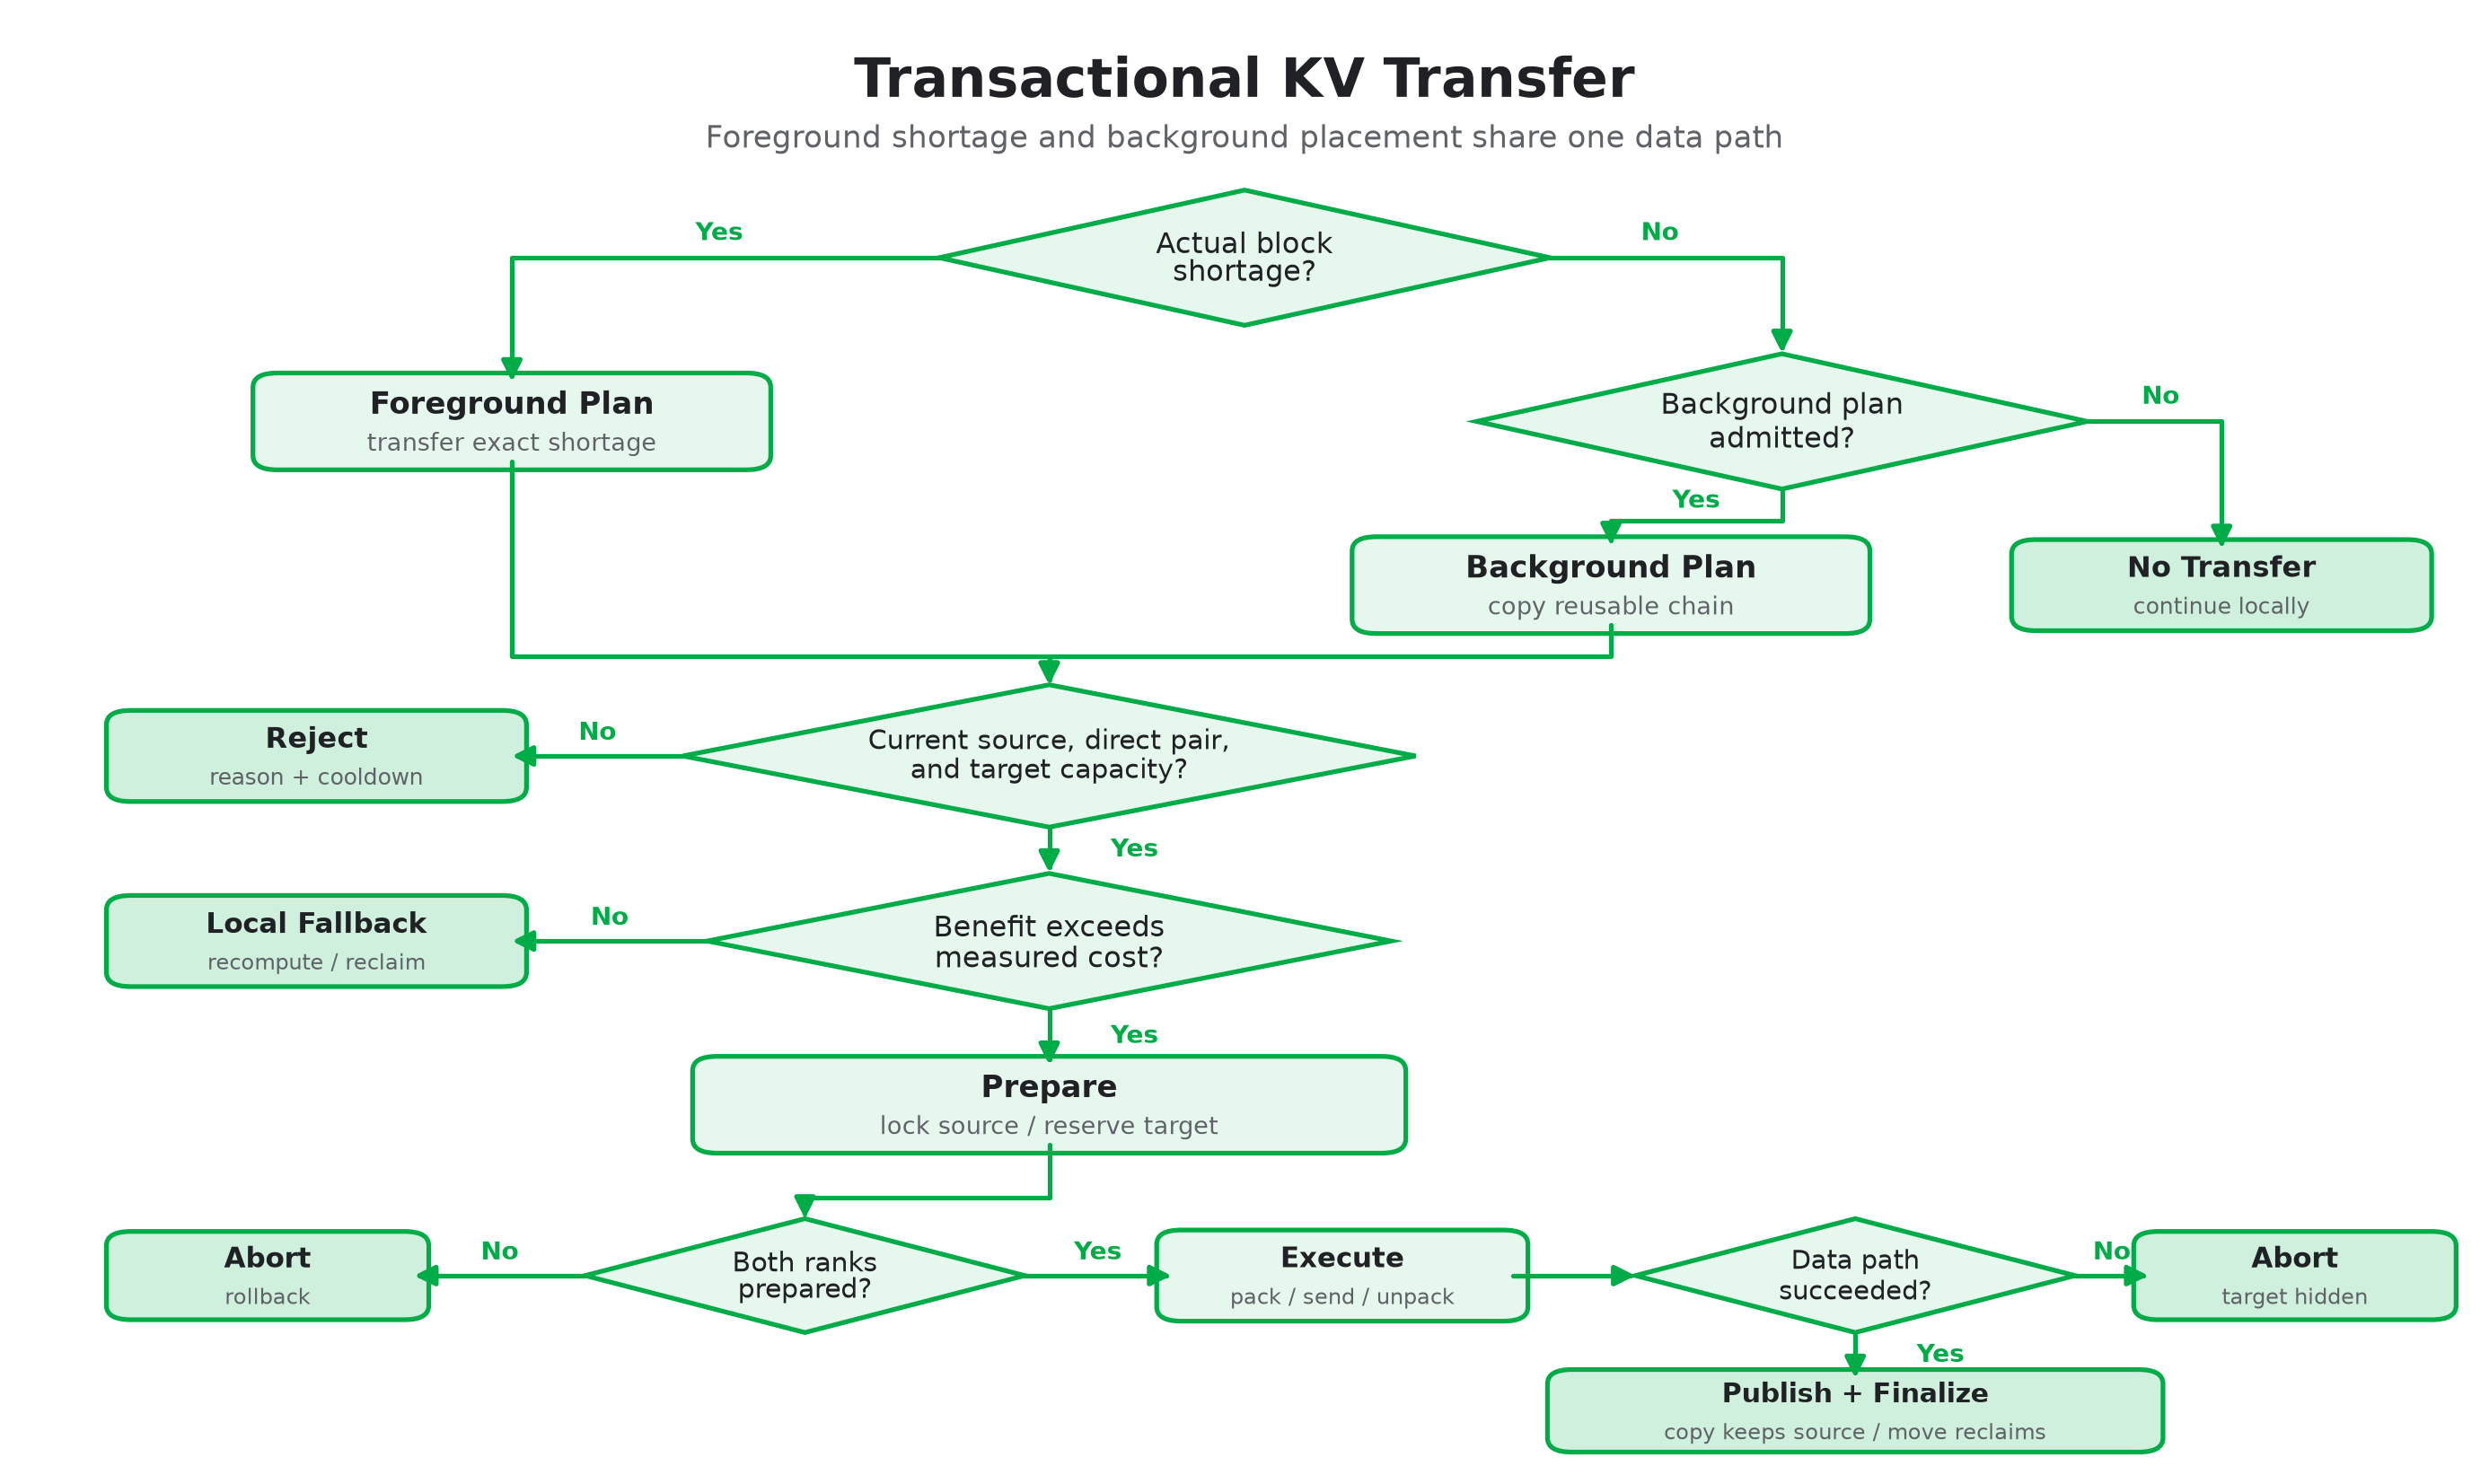
\includegraphics[width=0.9\textwidth]{fig_transfer_decision.png}
  \caption{Transactional transfer processes either a foreground block shortage or an admitted background chain through source validation, benefit checks, preparation, packed pair-local NCCL transfer, publication, and finalization. A failed phase follows the abort path without exposing the destination.}
  \label{fig:transfer-decision}
\end{figure*}

\subsection{Process and Ownership Model}

LLMEngine is the user-facing process. It launches one independent control-plane process and $N$ identical data-plane processes, including a data-plane process for rank~0. New sequences enter through LLMEngine, which sends sequence metadata and prefix hashes to the control plane through ControlPlaneClient. The control plane selects a rank before LLMEngine enqueues the complete sequence at the corresponding worker. Workers generally do not repeat global routing.

The control process owns GlobalScheduler and GlobalBlockManager. Each data-plane process owns one Local Scheduler, Local Block Manager, Model Runner, and CUDA device. This separation defines the ownership boundary. The global page table is the authoritative source of global metadata, whereas each Local Block Manager is authoritative for physical allocation, reference counts, readiness, and local KV tensors. Global Scheduler sends routing targets and transfer phases to each Local Scheduler. Each Local Block Manager sends a versioned snapshot to Global Block Manager after every relevant state change.

Figure~\ref{fig:arch} distinguishes three communication classes. The request and result path carries complete Sequence objects, generated tokens, and runtime measurements between LLMEngine and the selected worker. The metadata and control path carries versioned block and load snapshots to the control plane and carries transfer phases and heartbeat commands to the workers. The KV data path bypasses both LLMEngine and the control plane. The source Model Runner gathers a contiguous tensor from its local HBM cache, a pair-local NCCL communicator transfers the tensor over direct NVLink, and the destination Model Runner scatters the tensor into blocks reserved by the destination Local Block Manager.

LLMEngine also monitors and can restart the control process. Bidirectional heartbeat messages detect an unresponsive worker or control process, but provide neither consensus nor high availability. Worker state snapshots reconstruct the control metadata after a control-process restart. The current system cannot continue service after a launcher failure.

\subsection{Authoritative Global Metadata}

GlobalBlockManager maintains a page table $h \mapsto \{(g,b,\mathrm{generation},\mathrm{ready})\}$ that can record multiple replicas of the same hash. For each GPU, it also stores versioned snapshots of free, used, and evictable blocks, parent relationships, recency, and access frequency. Additional state includes routing reservations, blocks involved in active transfers, placement leases, worker epochs, and snapshot versions for rejecting stale updates.

Workers publish a complete snapshot after allocation, append, release, preemption, transfer publication, or a relevant cache-access change. GlobalBlockManager replaces each snapshot atomically at the granularity of one GPU. Reservations made during routing temporarily reduce the available capacity until the request commits the first prefill operation. This mechanism prevents a burst of routing decisions from consuming the same stale free-block count. Heartbeat reception does not advance page-table freshness, missing or stale snapshots trigger an explicit request for the complete state.

\subsection{KV-Aware Routing}
\label{sec:routing}

LLMEngine submits each ingress request to GlobalScheduler before assigning it to a worker. I denote this case by $s=-1$, every healthy replica is a candidate and has topology affinity $w(-1,g)=1$. For a worker-originated routing request with rank $s\geq0$, the candidate set contains $s$ and the directly connected NVLink partners of $s$. Let $\mathcal{N}_{\mathrm{NV}}(s)$ denote those partners. The topology affinity for this second case is
\begin{equation}
 w(s,g)=
 \begin{cases}
 2, & g=s,\\
 1, & g\in\mathcal{N}_{\mathrm{NV}}(s),\\
 0, & \text{otherwise}.
 \end{cases}
\end{equation}
Candidates with zero affinity are removed before cost evaluation. This distinction permits global admission-time routing while keeping worker-originated rerouting and physical data movement within configured direct pairs.

For candidate rank $g$, let $N$ denote the number of prompt tokens, $R$ the number of request blocks, $h_g$ the longest contiguous ready-prefix match, $S$ the block size, and $F_g$ the current number of free blocks. The required number of new blocks, block-rounded estimate of uncached prefill work, and reclamation pressure are
\begin{align}
 n_g &= \max(0,R-h_g), \\
 M_g &= \min(N,n_gS), \\
 A_g &= \max(0,n_g-F_g).
\end{align}
A rank is feasible only when the sum of its free and dependency-safe reclaimable capacity covers $n_g$. The token-equivalent queued work is
\begin{equation}
\begin{aligned}
 Q_g ={}& w_w(T_g^{\mathrm{wait}}+T_g^{\mathrm{pending}})
          + w_rT_g^{\mathrm{running}} \\
        &+ w_s(N_g^{\mathrm{running}}+N_g^{\mathrm{pending}}),
\end{aligned}
\end{equation}
with current defaults $w_w=1$, $w_r=0.25$, and $w_s=32$. GlobalScheduler then minimizes
\begin{equation}
 C_{\mathrm{route}}(g) = Q_g + w_pM_g + w_eA_gS,
\end{equation}
where $w_p=1$ and $w_e=0.5$ by default. Locality therefore enters through $h_g$ and directly reduces the estimated missing prefill work, it is not represented as an independent hit-rate reward subtracted from the cost. The prefix and topology score resolves ties between candidates with equivalent costs.

\begin{figure*}[t]
  \centering
  
\includegraphics[width=0.96\textwidth]{fig_routing_cost_model.png}
  \caption{Routing cost combines token-aware queued work, block-rounded uncached prefill, and dependency-safe reclamation pressure for each capacity-feasible rank. A bounded spill is permitted only when the prefix owner has sufficiently higher load and the additional recomputation cost remains within the configured limit.}
  \label{fig:routing-cost-model}
\end{figure*}

The router selects the feasible candidate with the lowest cost. It may bypass a prefix owner when the sequence pressure at that owner exceeds the pressure at another rank by a configured threshold and the additional recomputation cost remains bounded. When no candidate contains a reusable prefix, the router selects the rank with the lowest projected cost and sufficient effective capacity. This policy mitigates request skew and replica underutilization without changing the underlying data-parallel execution strategy.

\subsection{Local Allocation and Reclamation}

The Local Block Manager first searches for a matching ready local block and increments the reference count on a hit. When no match exists, it allocates a block identifier from a free deque and publishes the complete block only after Model Runner has written the KV data. Completed prefixes remain cacheable when their reference count reaches zero. Reclamation considers only dependency-safe leaf blocks, which prevents removal of an ancestor from orphaning a retained descendant. The replacement policy combines access frequency and recency. Live blocks with positive reference counts cannot be selected for move-based eviction, although they may be copied when replication is profitable. Figure~\ref{fig:kv-block-lifecycle} summarizes the normal local path and the transactional cross-GPU path.

\begin{figure*}[t]
  \centering
  
\includegraphics[width=0.98\textwidth]{fig_kv_block_lifecycle.png}
  \caption{A KV block moves through allocation, readiness, reference, caching, reservation, publication, and reclamation states under Local Block Manager ownership. Model Runner writes or transfers the physical K/V tensor, while blocks that are reserved or received but unpublished remain invisible to routing. Publication precedes copy or move finalization, and an abort preserves the source and releases the destination reservation.}
  \label{fig:kv-block-lifecycle}
\end{figure*}

The distinction between ``received'' and ``published'' defines the visibility boundary. A successful NCCL receive does not by itself create a routable replica. The destination must first record the complete hash chain and readiness state in its local snapshot, after which the control plane can expose the new location. Under copy semantics, a referenced source remains valid and is only unlocked. Under move semantics, reclamation is limited to an unreferenced and dependency-safe suffix. Partial or not-yet-ready local blocks bypass the cache and return directly to the free deque when released.

\subsection{Foreground Transfer}
\label{sec:fg-transfer}

Foreground transfer is demand-driven. If a block shortage of $k$ occurs during local prefill or decode append, the worker requests exactly $k$ blocks from the control plane rather than the complete block count of the request. GlobalScheduler selects a complete source chain and determines whether the operation is a move or a copy. After publication, a move may release a dependency-safe suffix at the source, whereas a copy retains the source and creates another replica. Pinned prefixes may be copied but cannot be released.

For $B$ blocks, $L$ layers, block size $S$, $H_{kv}$ KV heads, head dimension $D$, and $d$ bytes per element, the packed payload is $X=2BLSH_{kv}Dd$. For each logical NVLink pair $p$, the transfer microbenchmark provides the monotonic P95 data-path profile $\mathcal{P}_p=\{(X_i,Q^{95}_{p,i})\}$. A second profile $\mathcal{R}_p=\{(X_i,R^{95}_{p,i})\}$ records the P95 nonnegative dispatch-to-publication residual from completed serving transactions. The data-path prior and the static estimate are
\begin{align}
 T_{\mathrm{data}}^{p}(X) &= \operatorname{PWL}(X,\mathcal{P}_p), \\
 T_{\mathrm{static}}^{p}(X) &= \bigl(R^{95}_{p}(X)+I T_{\mathrm{data}}^{p}(X)\bigr)w_x.
\end{align}
The model uses linear interpolation between adjacent samples. Below the measured range it uses the nearest boundary, above the range it extends the slope of the final measured segment. Let $b(B)=2^{\lceil\log_2 B\rceil}$ be the size bucket. Completed source operations and dispatch-to-publication observations update separate nonnegative residual EWMAs $\Delta^{src}_{p,b}$ and $\Delta^{place}_{p,b}$. The admission estimate remains conservative:
\begin{equation}
\begin{aligned}
 T_{\mathrm{xfer}}=\max\bigl\{&
 T_{\mathrm{prior}}^{p},\\
 &(T_{\mathrm{data}}^{p}+\Delta^{src}_{p,b})w_x,\\
 &(I T_{\mathrm{data}}^{p}+\Delta^{place}_{p,b})w_x
 \bigr\}.
\end{aligned}
\end{equation}
Here $I=1.2$ is the interference multiplier and $w_x$ is the configured transfer-cost weight. When the calibrated residual profile is available, $T_{\mathrm{prior}}^{p}=T_{\mathrm{static}}^{p}$. When it is unavailable, the implementation uses a zero-residual fallback until a completed placement observation is available, it then uses the larger of the data-path estimate and the online placement estimate. The residual profiles and EWMAs are nonnegative, so an unusually fast observation cannot make admission more aggressive than the calibrated data-path prior. Foreground saved work uses discounted historical chain reuse $\widehat{R}$, whereas background admission counts only the first avoidable cold prefill because the destination cache becomes warm after a miss:
\begin{align}
 T_{\mathrm{save}}^{fg} &= \widehat{R}BS t_{\mathrm{prefill}}, \\
 T_{\mathrm{save}}^{bg} &= BS t_{\mathrm{prefill}}(g_{dst}).
\end{align}
A plan is admitted only when the source generations and target capacity remain valid and $T_{\mathrm{save}} \ge \rho T_{\mathrm{xfer}}$ for the configured safety ratio $\rho$. Repeated background candidates with the same low-benefit or insufficient-capacity signature enter a negative cache until the signature changes.

\begin{figure*}[t]
  \centering
  
\includegraphics[width=0.96\textwidth]{fig_transfer_cost_model.png}
  \caption{Transfer admission compares expected saved prefill time with a pair-specific P95 latency profile and runtime residuals for the corresponding size bucket. Foreground and background paths estimate saved work differently but share the same validity, capacity, and benefit-ratio checks.}
  \label{fig:transfer-cost-model}
\end{figure*}

\subsection{Background Placement}
\label{sec:bg-transfer}

Background placement addresses predictable future reuse rather than an immediate allocation failure. Workers report cumulative access counts and parent hashes for ready blocks. The control plane selects maximal chains by their deepest hot leaf and reconstructs all resident ancestors in prefix order. Route-hit counts provide an online trigger. When ingress has information about queued requests that have not yet been submitted, it can also provide a forecast that maps hashes to future demand. When a demand forecast is available, predicted reuse is capped by that forecast. Otherwise, predicted reuse is estimated from the minimum access count along the chain after subtraction of observed uses and application of a conservative discount. This signal creates only a candidate. Admission further requires the absence of an existing destination replica, completion of cooldown and idle-pressure checks for the directed pair, and sufficient target capacity.

Compatible candidates are deduplicated and batched for each directed NVLink pair. The default configuration limits one candidate chain to eight blocks and a coalesced pair payload to 128 blocks. These limits are upper bounds rather than fixed transfer sizes. Background admission counts at most the first avoidable cold prefill at the destination because, in the absence of an intervening eviction, the destination GPU becomes warm after its first miss. The model therefore does not multiply the expected benefit by every forecast request. A placement lease is created only after publication. Explicit quotas for the source and replica distribute subsequent matching requests across both GPUs, which couples speculative placement with routing rather than merely duplicating data.

The load-skew workload exercises background placement without rank hints. A warm-up phase creates one instance of each hot prefix, and a subsequent burst reuses those prompt identities. The control plane selects source and target ranks from prefix ownership, direct topology, capacity, and load state, placement leases later expose completed replicas to routing.

\subsection{Transactional Transfer Protocol}

A transfer plan has four externally visible phases. During preparation, the destination reserves concrete free block IDs and both workers record the plan state, routing cannot observe the new location. During execution, the source and destination issue matching NCCL point-to-point operations. The source uses indexed selection to gather physical blocks into one contiguous tensor of shape $[L,2,B,S,H_{kv},D]$, which represents layers, K/V, transferred blocks, block tokens, KV heads, and head dimension. A pre-initialized pair-specific process group transfers the tensor once. The destination receives a buffer of the same shape and uses indexed copies to scatter the data into the reserved physical blocks. Hashes, generations, and destination block IDs remain metadata in the control protocol and do not enter the NCCL tensor payload.

During publication, the destination marks the received blocks as ready and publishes a versioned snapshot. Only after this step can the control plane expose the new page-table location or placement lease. During finalization, a move verifies the hash and generation of each source block before releasing the specified suffix, whereas a copy retains the source. A failure during preparation or execution aborts the transaction, releases all reservations, and preserves the authority of the source.

The protocol is idempotent for each plan ID and phase. Per-client receive locks serialize consumption of response queues, one event loop serializes mutations of control-plane state, and block mutations remain single-threaded within each worker. These measures protect metadata transactions without introducing a global lock on the inference fast path.

\section{Implementation}
\label{sec:impl}

\sys{} extends single-GPU inference engine Mini-vLLM using Python and PyTorch. Table~\ref{tab:modules} summarizes the implementation.

\begin{table}[t]
  \centering
  \caption{Principal Implementation Modules}
  \label{tab:modules}
  \footnotesize
  \setlength{\tabcolsep}{3.5pt}
  \begin{tabular}{@{}L{0.34\linewidth}L{0.60\linewidth}@{}}
    \toprule
    Module & Responsibility \\
    \midrule
    LLM engine & Request ingress, process launch and supervision, completion aggregation \\
    Control plane & Protocol handling, clients, authoritative event loop, heartbeat processing \\
    Global scheduler & Cost-based routing and transfer-plan decisions \\
    Global block manager & Global page table, snapshots, reservations, candidate tracking \\
    Data plane & Per-rank worker loop and transfer-phase execution \\
    Local scheduler & Local prefill and decode admission, shortage detection \\
    Local block manager & Physical blocks, prefix cache, references, reclamation \\
    Model runner & Model execution, KV tensors, metrics, transfer interface \\
    KV transfer & Packed NCCL movement of GPU-to-GPU payloads \\
    \bottomrule
  \end{tabular}
\end{table}

\subsection{Testing Strategy}

I conduct unit tests for each engine module. Table~\ref{tab:tests} summarizes the coverage.
The tests use fake components to obtain deterministic control decisions.

\begin{table}[t]
  \centering
  \caption{Test Design and Coverage}
  \label{tab:tests}
  \footnotesize
  \setlength{\tabcolsep}{3.5pt}
  \begin{tabular}{@{}p{0.30\linewidth}p{0.62\linewidth}@{}}
    \toprule
    Test group & Covered behavior \\
    \midrule
    Block managers & Allocation and release, chain reuse, LFU/LRU leaves, generations, snapshots \\
    Global scheduler & Hit, miss, and capacity routes, load bypass, direct-pair filtering, move and copy plans \\
    Control plane & Epochs, stale updates, reservations, leases, idempotent phases, heartbeats, concurrency \\
    Data plane/engine & Queue protocol, master-first ingress, worker and control lifecycles, result aggregation \\
    KV transfer & Shape and byte accounting, copy and move primitives, two-rank NCCL equality, deadlock detection \\
    Model runner & KV layout, prefill and decode preparation, dtype consistency, transfer adapters \\
    Benchmarks & Workloads, schemas, metrics, confidence intervals, plotting, transfer-profile construction and validation \\
    End-to-end & Multi-process request completion and optional CUDA/NCCL integration \\
    \bottomrule
  \end{tabular}
\end{table}

\section{Evaluation}
\label{sec:eval}

The evaluation addresses four questions: (Q1) Does KV-aware routing improve service under long shared prefixes? (Q2) What latency and bandwidth does the transfer data path provide? (Q3) Does background placement execute under load skew, and what serving trade-off does it create? (Q4) Can foreground offloading work safely and efficiently under memory skew? Q1 is the primary end-to-end performance claim. Q2-Q4 establish data-path correctness, protocol behavior, and the boundary at which completed transfer does not yield an incremental serving gain.

\subsection{Setup and Methodology}

The evaluation uses six 24~GiB GeForce RTX 3090 GPUs selected from a host with seven GPUs. The measured topology contains three direct pairs: physical GPUs $(0,1)$, $(3,4)$, and $(5,6)$. The benchmark exposes these devices as logical pairs $(0,1)$, $(2,3)$, and $(4,5)$, respectively. Both the NVLink topology and peer-access matrices report a direct path for each selected pair and no direct path between pairs. The topology label NV4 denotes a bonded set of four links. RTX 3090 uses the third-generation NVLink interface of the GA102 architecture, each link provides 14.0625~GB/s in each direction, so one four-link pair has a theoretical peak of 56.25~GB/s per direction and 112.5~GB/s in aggregate across both directions~\citep{NVIDIAAmpereGA102}. The KV-transfer workload is unidirectional and is therefore compared with the 56.25~GB/s limit.

I evaluate Qwen3-0.6B and Qwen3-1.7B using BF16. Both models contain 28 layers, eight KV heads, and a head dimension of 128, which yields the same 114,688 KV bytes per token. The KV block size is 256 tokens. Each system experiment uses a fixed KV block budget per worker and five repetitions with seed~0. EOS termination is disabled. Routing generates 64 output tokens, memory skew generates 16, and load skew generates 8 to emphasize admission and prefill behavior. Goodput uses the workload-specific configured E2E SLA.

Every JSON artifact records the command, resolved model configuration, Git state, values from individual trials, 95\% confidence intervals, and per-rank statistics. Each scenario runs in fresh processes, so cache contents do not persist across scenarios. The complete artifact set corresponds to the result dated 20260727T231622Z.

\subsection{Synthetic Dataset Profiling}

The study uses deterministic synthetic prompts rather than a public conversational trace. Each prompt applies the Qwen chat template to a repeated instruction body and a group-specific suffix. This construction makes the amount and ownership of reusable KV state explicit. Table~\ref{tab:datasets} profiles the tokenized inputs and phase structure. Dataset-level profiling is necessary because request hit rate alone does not quantify the number of reusable prompt tokens.

I report two intrinsic trace metrics before applying any system policy. Let $m_i$ be the number of complete, contiguous prefix blocks of request $i$ whose cumulative hashes appeared in an earlier request, $B$ the block size, and $T_i$ the prompt length. Request prefix sharing is $\sum_i \mathbb{1}[m_i>0]/N$, while token prefix sharing is $B\sum_i m_i/\sum_i T_i$. These values are ordered-replay upper bounds under unlimited cache capacity and perfect placement, the calculation excludes partial tail blocks. Runtime request hits and cached-token ratio are reported separately.

\begin{table*}[t]
  \centering
  \caption{Synthetic Workload Profiles}
  \label{tab:datasets}
  \scriptsize
  \setlength{\tabcolsep}{2pt}
  \renewcommand{\arraystretch}{1.08}
  \begin{tabular}{@{}L{0.08\textwidth}L{0.06\textwidth}L{0.22\textwidth}L{0.10\textwidth}L{0.07\textwidth}L{0.10\textwidth}L{0.05\textwidth}L{0.16\textwidth}@{}}
    \toprule
    Workload & Requests & Prefix Construction & Prompt Tokens & Req. Share & Token Share & Window & Purpose \\
    \midrule
    Routing & 192 & 16 recurring groups, first request in each group is cold, shared prefix length is 1x, 3x, or 5x & 365,880 / 1,084,728 / 1,803,576 & 91.67\% & 86.20\% / 91.38\% / 89.93\% & 16 & Test locality-aware routing. \\
    Load skew & 192 & Three long hot groups, three warm-ups followed by 189 hot reuses & 1,444,344 & 98.44\% & 97.15\% & 96 & Test background placement. \\
    Memory skew & 72 & Six session warm-ups, 30 anchor/cold pressure requests, and 36 session reuses & 486,554 & 91.67\% & 72.29\% & 48 & Test foreground offloading. \\
    \bottomrule
  \end{tabular}
\end{table*}

\subsection{Baselines and Metrics}

I define five normalized scenarios. The single-gpu scenario runs one replica. The multi-gpu scenario uses static round-robin data parallelism. The multi-gpu-kv-routing scenario enables global routing but disables transfer. The multi-gpu-kv-transfer scenario retains round-robin request placement and enables transfer. The multi-gpu-lmpool scenario enables both mechanisms. All multi-GPU scenarios use the same KV block budget per worker.

These scenarios are controlled internal ablations. They isolate the incremental effects of routing and transfer while holding model execution, KV capacity, and request generation constant. They are not direct comparisons with production vLLM, SGLang, Mooncake, or LMCache deployments, so the evaluation does not establish superiority over those systems.

The primary metrics are output throughput, SLA goodput, mean TTFT, decode time per output token (TPOT), mean and P90 E2E latency, and uncached prefill tokens. For request $i$, let $s_i$ be the submission time, $f_i$ the first-token time, $c_i$ the completion time, and $N_i$ the number of output tokens. I compute $\mathrm{TTFT}_i=f_i-s_i$ and $\mathrm{TPOT}_i=(c_i-f_i)/(N_i-1)$. Requests with $N_i=1$ have no decode interval and are excluded from TPOT statistics. This definition removes queueing and prefill time from the decode-rate metric. I distinguish control-plane request hits, route-to-owner hits, data-plane local request hits, and cached-token ratio. Transfer counters report the number of blocks, payload bytes, copy and move operations, protocol outcomes, and estimated and observed costs. Per-rank distributions of requests, tokens, execution time, and utilization expose load concentration.

For a metric measured in $R$ complete repetitions, I report the sample mean $\bar{x}=R^{-1}\sum_{r=1}^{R}x_r$ and the two-sided 95\% confidence interval $\bar{x}\pm t_{0.975,R-1}s/\sqrt{R}$, where $s$ is the sample standard deviation. The experiments use $R=5$, for which $t_{0.975,4}=2.776$. For a tail metric such as P90 E2E, $x_r$ is the request-level P90 computed within repetition $r$, the interval is then computed across the five repetition-level P90 values. These intervals quantify run-to-run variation under the fixed setup, not the request-level latency distribution or variation across models and hardware.

\begin{figure*}[t]
  \centering
  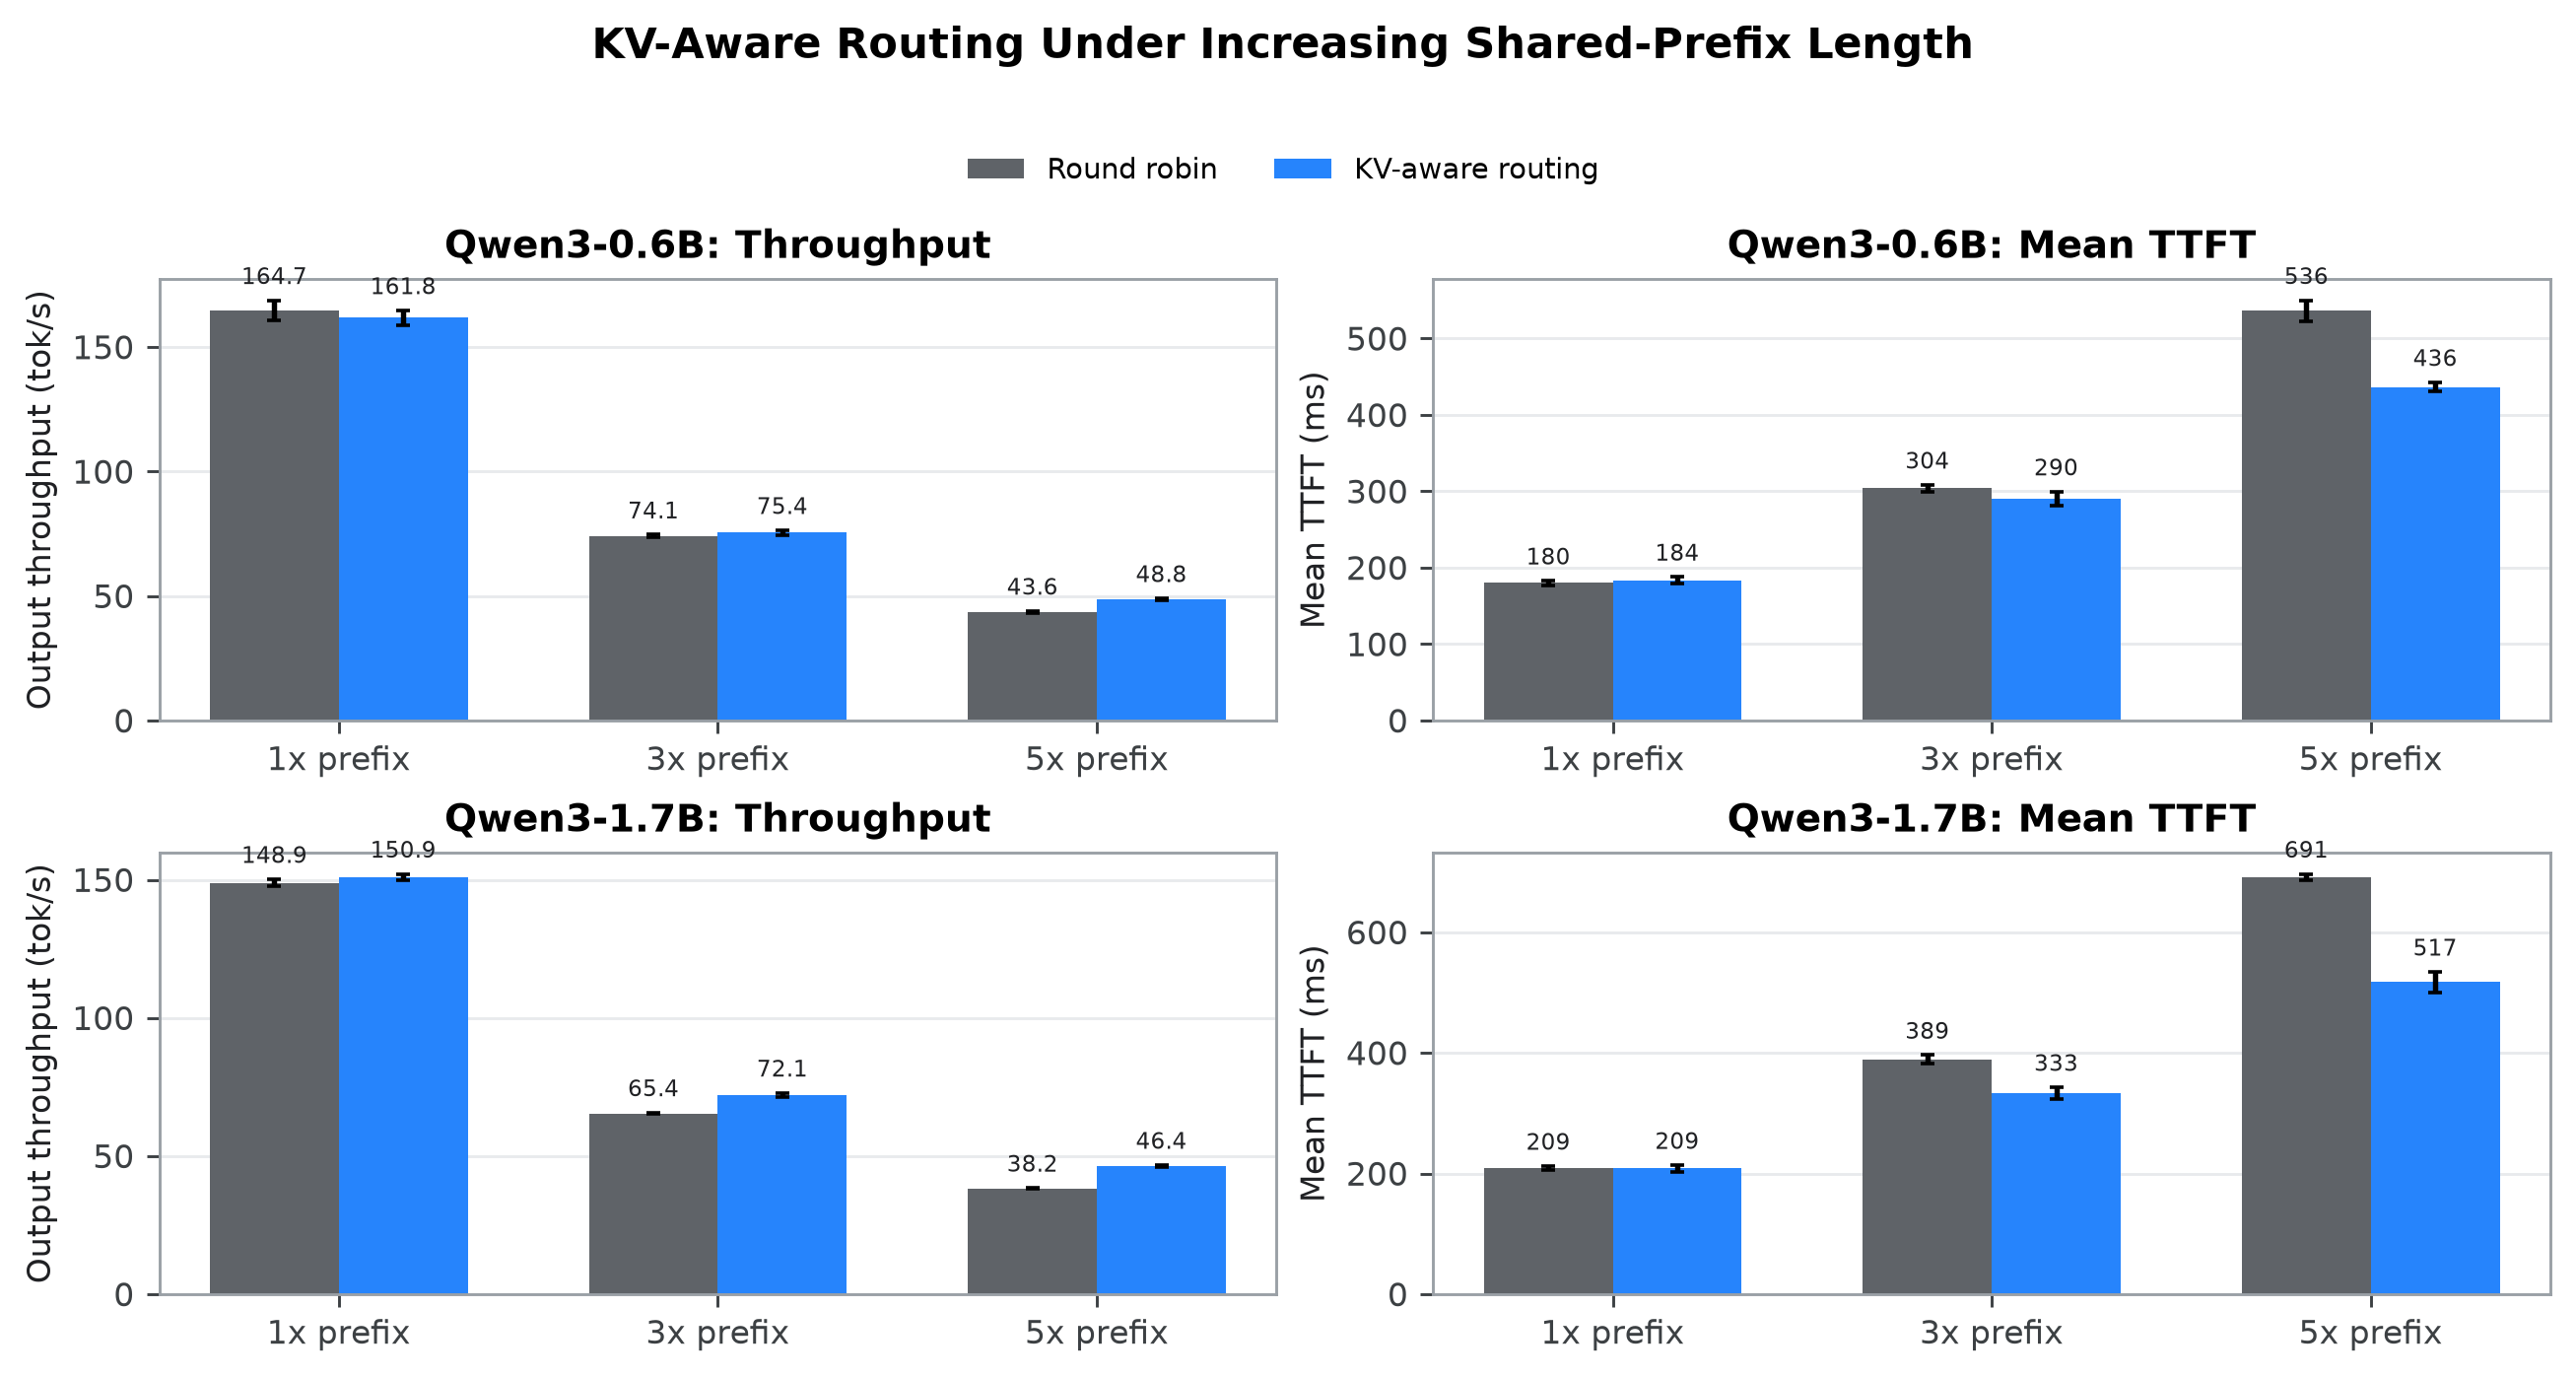
\includegraphics[width=\textwidth]{fig_suite_routing.png}
  \caption{Routing Results Under Increasing Shared-Prefix Length}
  \label{fig:suite-routing}
\end{figure*}

\begin{figure*}[t]
  \centering
  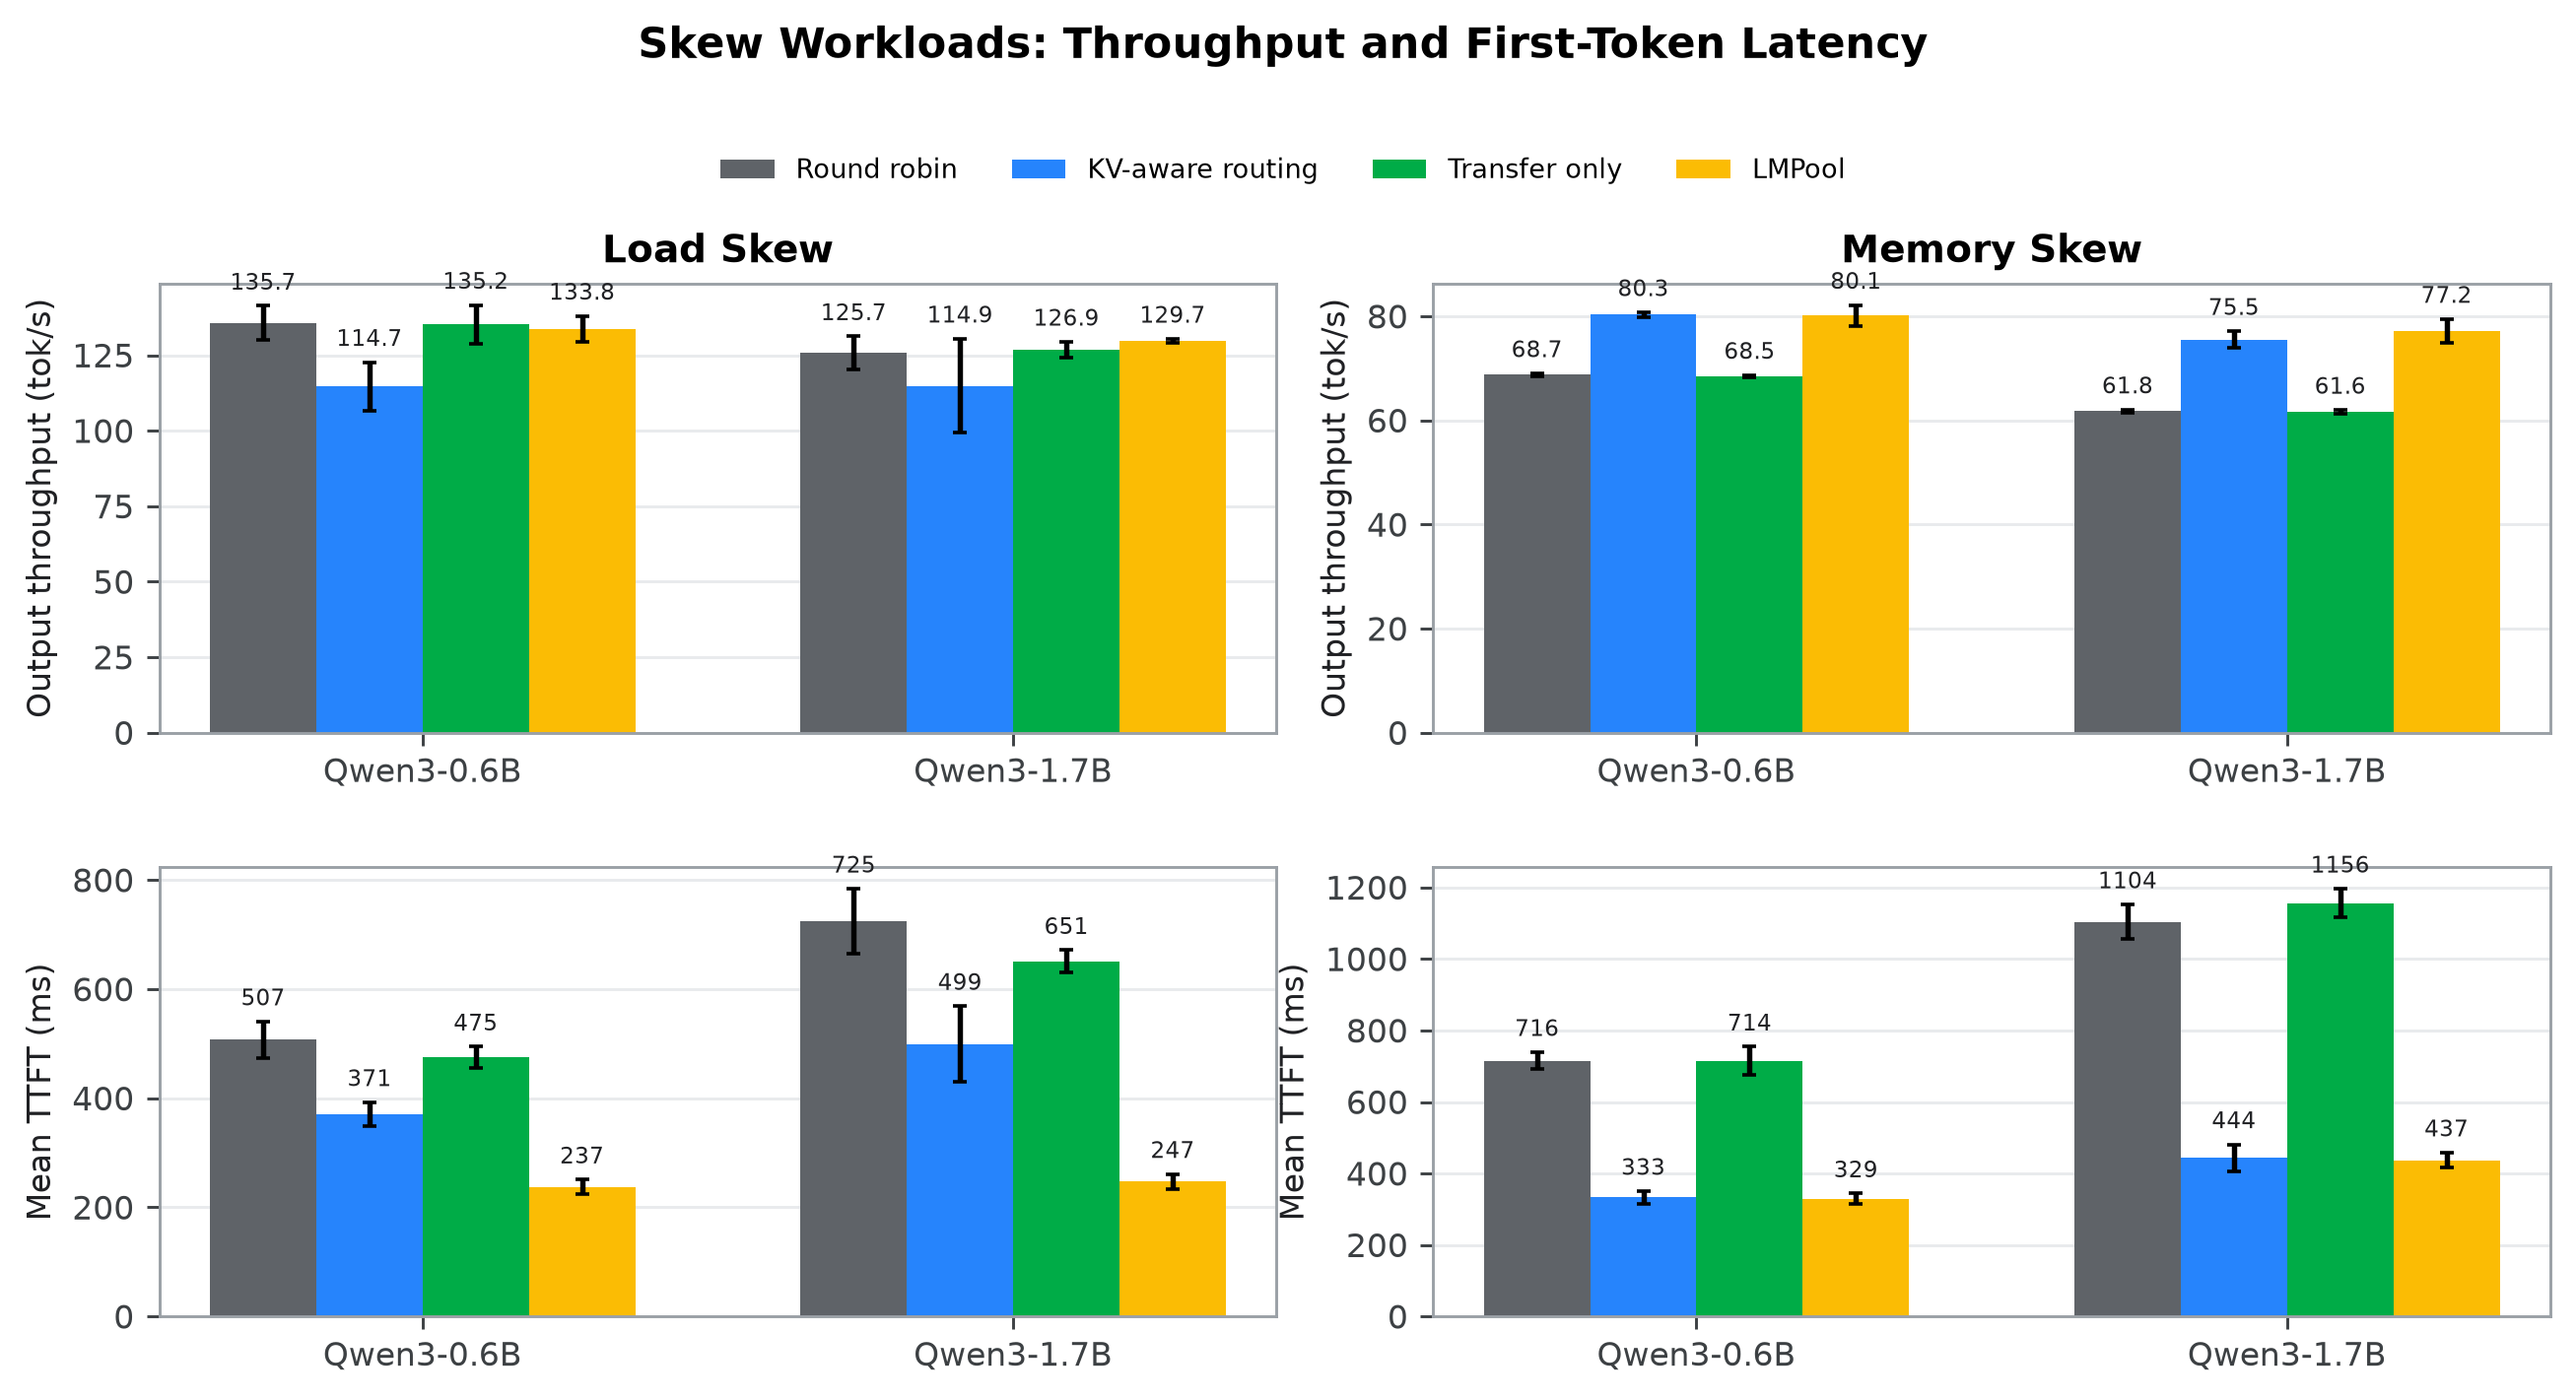
\includegraphics[width=\textwidth]{fig_suite_skew.png}
  \caption{Throughput and Mean TTFT on Load-Skew and Memory-Skew Workloads}
  \label{fig:suite-skew}
\end{figure*}

\begin{figure*}[t]
  \centering
  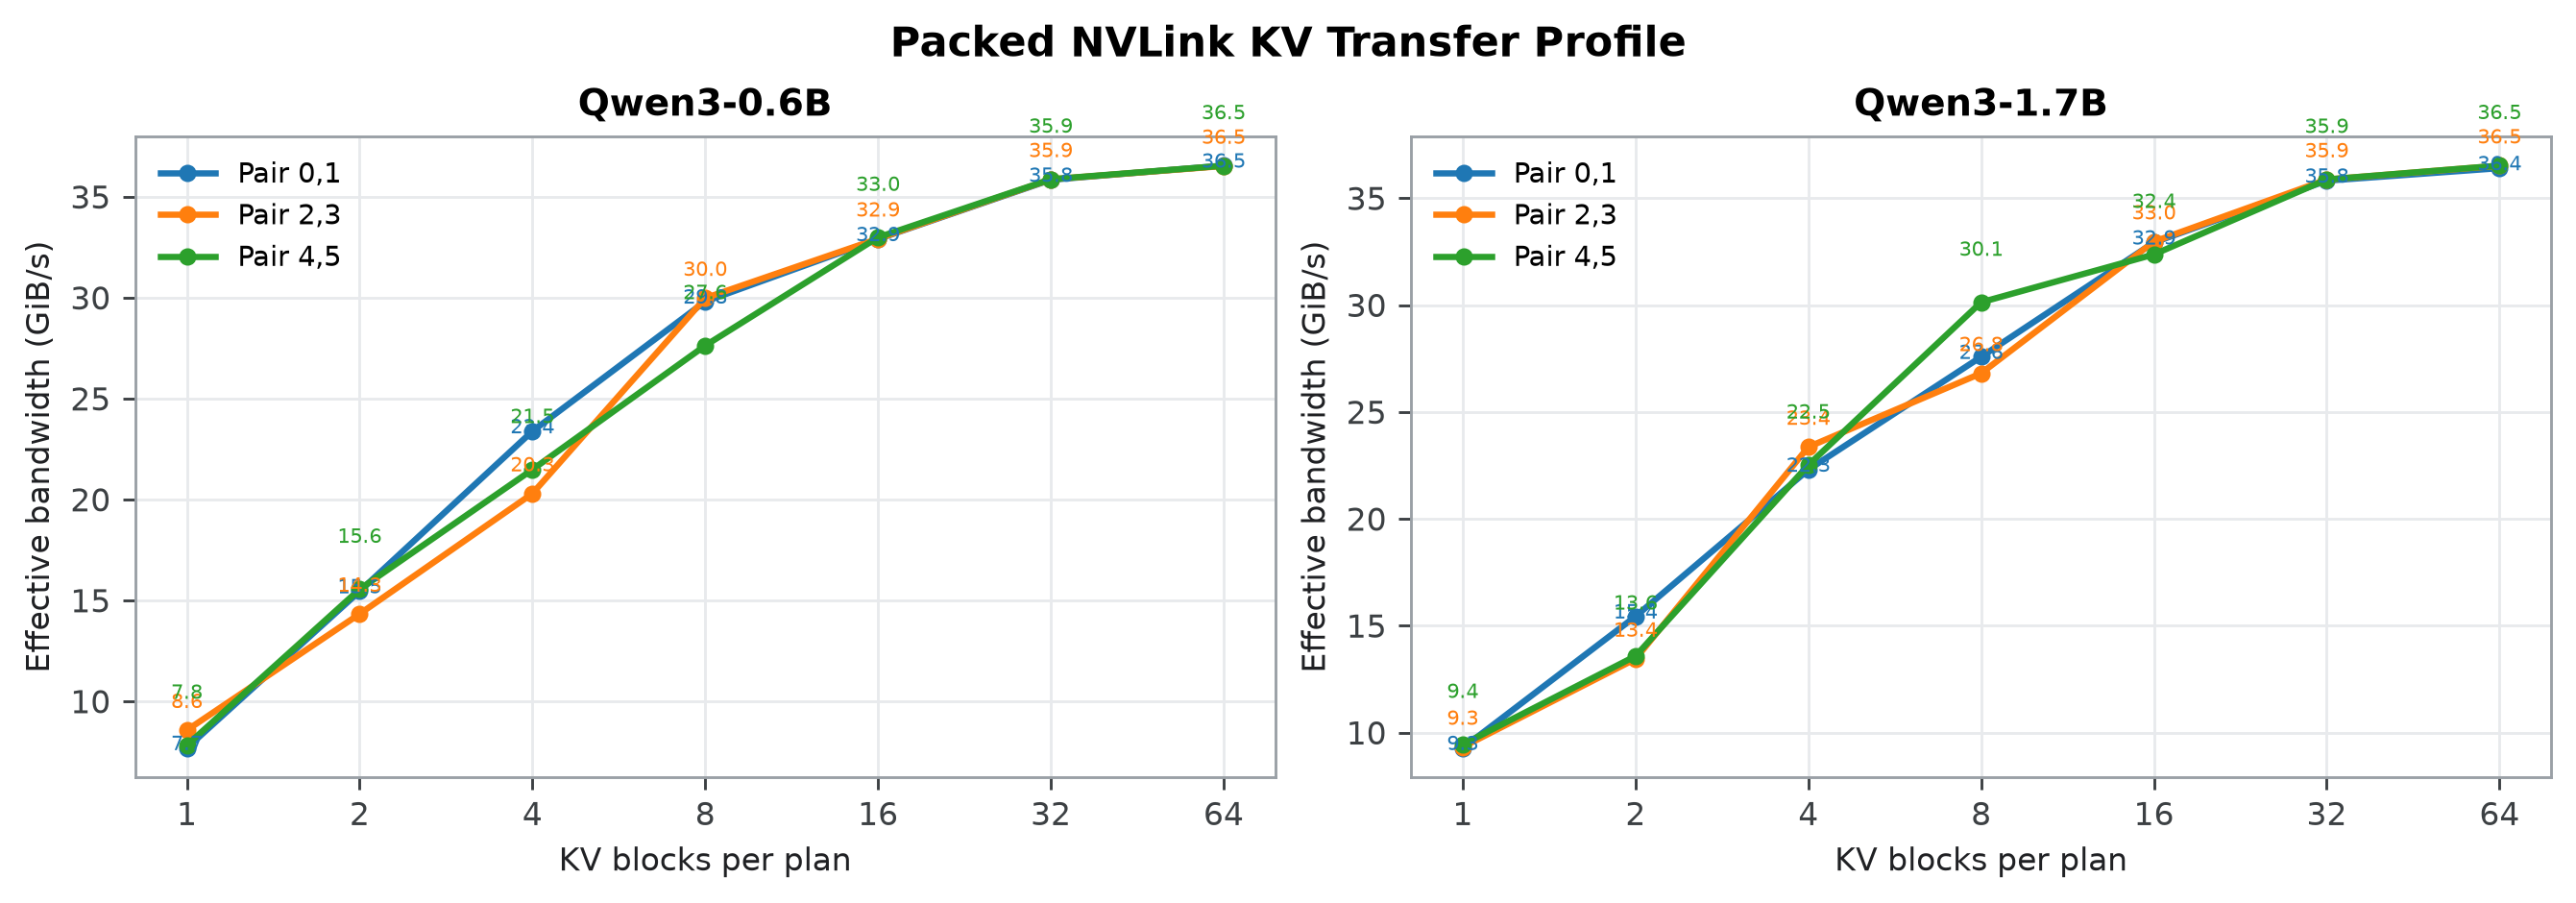
\includegraphics[width=0.92\textwidth]{fig_suite_transfer_profile.png}
  \caption{Packed NVLink KV Transfer Profiles across Direct GPU Pairs}
  \label{fig:suite-transfer-profile}
\end{figure*}

\subsection{Q1: Does KV-aware routing improve service under long shared prefixes?}

\paragraph{Routing Benefit Grows With Prefix Length.} Figure~\ref{fig:suite-routing} reports five-trial means and 95\% confidence intervals. At 1x, routing does not improve service throughput: Qwen3-0.6B changes from 164.7 to 161.8~tok/s and Qwen3-1.7B from 148.9 to 150.9~tok/s. TTFT is also unchanged or slightly higher. The matched prefix is too short for the avoided prefill to dominate normal scheduling variation. At 3x and 5x, the avoided work becomes large enough to change service metrics. For Qwen3-0.6B at 5x, routing increases throughput from 43.63 to 48.77~tok/s, reduces mean TTFT from 536 to 436~ms, reduces mean E2E from 2,743 to 2,338~ms, and reduces P90 E2E from 3,977 to 3,140~ms. It also reduces uncached prefill tokens from 884,997 to 354,821. For Qwen3-1.7B at 5x, throughput increases from 38.22 to 46.38~tok/s, mean TTFT decreases from 691 to 517~ms, mean E2E decreases from 3,156 to 2,479~ms, and P90 E2E decreases from 4,903 to 3,649~ms. The corresponding uncached prefill reduction is 61.0\%. The improvements exceed the reported run-to-run confidence intervals at the longer prefix settings.

\paragraph{Locality Is Converted Into Saved Computation.} The request-level sharing bound is constant at 91.67\% across the routing sweep, but token sharing rises because the shared prefix becomes longer. The router does not add a separate reward for hit rate. Instead, a longer contiguous match lowers the missing prefill term in the route cost, so the same locality becomes a direct reduction in scheduled compute. The result is strongest at 5x, where both models improve throughput and all reported latency metrics rather than only cache-hit counters.

\subsection{Q2: What latency and bandwidth does the transfer data path provide?}

\paragraph{The Data Path Preserves KV Semantics.} The microbenchmark transfers the K and V tensors of every layer between two ranks and validates the destination byte for byte. It verifies the packed tensor shape, byte count, dtype path, and receive-side contents for every measured pair and plan size. Passing this check establishes that the bandwidth measurements correspond to the same packed tensors consumed by the serving path rather than to an unrelated communication primitive. The microbenchmark alone does not establish an end-to-end serving benefit, because it does not include future reuse, queueing, or interference with model execution.

\paragraph{Larger Plans Amortize Fixed Data-Path Cost.} Figure~\ref{fig:suite-transfer-profile} reports the effective bandwidth of the same packed tensor that the serving path consumes. The profile covers 1/2/4/8/16/32/64-block plans on three direct pairs for both models, validates every destination byte for byte, and initializes pair-specific P95 piecewise-linear latency curves. A 64-block payload is about 1.75~GiB and has a mean critical-path latency near 48~ms. Its bandwidth is higher than that of the small plans because gather, packing, communicator synchronization, and scatter are amortized over more K/V data, the curve should not be read as a raw-link measurement. Runtime plans are not restricted to the sampled sizes: the scheduler interpolates the profile by payload and updates pair-by-size residuals from completed operations.

\subsection{Q3: Does background placement execute under load skew, and what serving trade-off does it create?}

\paragraph{The Load-Skew Trace Exercises The Intended Path.} The 98.44\% request-sharing load-skew trace leaves target capacity after three warm-up requests. On both models, transfer-only and full \sys{} complete three background placements and copy 87 blocks. Full \sys{} then routes 95 requests through placement leases, while transfer-only retains round-robin admission. This result establishes that the copied prefixes become visible to later routing decisions rather than merely completing a data-path operation.

\paragraph{TTFT Improves, While Decode Can Limit E2E.} For Qwen3-0.6B, \sys{} reduces mean TTFT from 507~ms under round robin to 237~ms, and reduces uncached prefill tokens from 152,568 to 41,208. Relative to routing-only, the same configuration reduces TTFT from 371 to 237~ms and raises throughput from 114.7 to 133.8~tok/s, which is consistent with lease routing using the copied replicas rather than leaving requests at their original owners. It remains slightly below round-robin throughput, 133.8 versus 135.7~tok/s, and has higher mean E2E, 2,754 versus 2,540~ms. For Qwen3-1.7B, \sys{} increases throughput from 125.7 to 129.7~tok/s, reduces TTFT from 725 to 247~ms, and reduces P90 E2E from 4,850 to 4,071~ms, mean E2E increases slightly from 2,782 to 2,840~ms. The E2E trade-off is consistent with the mean TPOT increase: copied-prefix placement reduces prefill delay, but the current decode scheduler can incur more contention after the first token. The load-skew result therefore supports background-copy correctness and a strong TTFT benefit, but not a universal mean-E2E claim.

\subsection{Q4: Can foreground offloading work safely and efficiently under memory skew?}

\paragraph{Offloading Is Verified Functionally, But Does Not Necessarily Improve Serving Performance Only By Itself} In memory skew, the 0.6B full-system result reports 35 released source blocks, two copy operations, and a true offload verification flag. Transfer-only remains close to round robin, with 68.47 versus 68.75~tok/s and 714 versus 716~ms TTFT, so movement alone does not remove enough work to improve service. Routing is the dominant improvement: it raises throughput from 68.75 to 80.30~tok/s and reduces TTFT from 716 to 333~ms by selecting existing local prefix chains. Adding the move path yields 80.11~tok/s and 329~ms, which is statistically close to routing-only. The 1.7B result records moved blocks but does not satisfy the complete offload verification predicate. Its full-system throughput and latency are close to routing-only, with confidence intervals that overlap. Thus the experiment verifies a safe capacity-release transaction without demonstrating an incremental throughput gain. The paper therefore uses memory skew as an implementation and safety result, not as evidence that transfer-out improves serving performance. This negative boundary is important because memory pressure alone does not ensure a reusable, feasible, and sufficiently valuable transfer plan.

\section{Discussion, Limitations, and Future Work}
\label{sec:limitations}

The study uses one host, six consumer GPUs, and two models with fewer than two billion parameters and identical KV geometry. It does not evaluate scale-out beyond six GPUs or sensitivity to the 256-token KV block size. Smaller blocks may change fragmentation, metadata cost, transfer-plan size, and batching efficiency. Larger models alter the ratio between computation and transfer, while larger NVLink fabrics alter candidate selection.
An NVSwitch fabric requires separate evaluation: it enlarges each source GPU's feasible target set, and concurrent transfers contend for a shared fabric rather than independent pair-local links. Pair-specific profiles measured on the current topology therefore do not establish routing or admission behavior on an all-to-all NVSwitch domain.
The reported results should not be extrapolated directly to RDMA or PCIe-only clusters.

The internal ablations provide a controlled comparison of mechanisms but do not compare complete production serving stacks on production traces. Differences in kernels, schedulers, prefix indexes, connector implementations, and workloads prevent the reported improvements from being interpreted as superiority over vLLM, SGLang, Mooncake, or LMCache.

Versioned snapshots, transactional transfers, heartbeats, and control-process restart preserve metadata consistency and support failure detection. They do not implement replicated consensus. A launcher failure stops the service, and a worker failure can remove the physical cache stored by that worker.

The model- and pair-specific size curve and bucketed EWMA capture payload scale and observed serving overhead. The current runner initializes the static estimate from the pair-specific P95 data-path profile and a measured transaction residual. It uses a zero-residual fallback only until a placement observation is available. The evaluation does not report held-out prediction error or sensitivity to the safety ratio and EWMA update. The cost model also does not explicitly condition on concurrent kernels, GPU clock rates, or link contention. Rapid changes in compute state can therefore lead to inaccurate estimates.

Future work should compare against production serving engines under the same model, arrival process, and KV budget, and should vary model size, KV geometry, block size, and GPU count with production traces.
It should also evaluate an eight-GPU NVSwitch domain, including concurrent transfer profiles, topology-aware candidate selection over a larger target set, and end-to-end scaling under shared-fabric contention.
The transfer study should report held-out prediction error and ablate the piecewise-linear profile, EWMA correction, safety ratio, and no-gate policy. A production deployment would also require replicated control metadata and launcher failover rather than the current single-control-process recovery model.

\section{Related Work}
\label{sec:related}

\subsection{LLM Serving and Prefix Caching}

Orca introduced iteration-level scheduling for transformer serving~\citep{ORCA}. PagedAttention in vLLM virtualizes KV allocation into blocks~\citep{vLLM}, while RadixAttention in SGLang organizes reusable prefix state for structured programs~\citep{SGLang}. Sarathi-Serve uses chunked prefill to control interference between prefill and decode~\citep{SarathiServe}. DistServe separates the two phases and optimizes goodput under TTFT and TPOT constraints~\citep{DistServe}. These systems establish the context for local execution and scheduling. In contrast, \sys{} studies admission-time placement among data-parallel replicas that can copy KV blocks over direct NVLink.

\subsection{Cluster Orchestration}

Ray~\citep{Ray} and Kubernetes~\citep{Kubernetes} manage resource allocation, worker placement, scaling, and lifecycle at cluster or replica granularity. Ray schedules distributed tasks and actors, while Kubernetes schedules and maintains containers. They can provide an outer deployment layer for \sys{}, but do not natively maintain prefix-level KV ownership, route requests from contiguous ready-prefix chains, or admit transactional KV movement. \sys{} is therefore complementary to cluster orchestration: an orchestrator manages replica lifecycle, whereas \sys{} manages request and KV placement within a serving group.

\subsection{Distributed and Tiered KV Caches}

Mooncake introduced a KV-cache-centric disaggregated architecture that exchanges distributed storage capacity for reduced prefill computation~\citep{Mooncake}. The newer integration between vLLM and Mooncake Store pools KV state across instances through GPUDirect RDMA and a distributed DRAM/SSD service. The official evaluation on agentic traces reports 3.8$\times$ higher throughput, 46$\times$ lower P50 TTFT, and 8.6$\times$ lower E2E latency on 12 GB200 GPUs. A synthetic scale-out experiment maintains a cache hit rate above 95\% at 60 GPUs~\citep{MooncakeStore}. The integration can query block hashes during scheduling, while the authors identify complete cache-aware routing and multi-node NVLink support as future work. PegaFlow instead places cache ownership in a long-lived Rust service and combines pinned host DRAM, one-sided RDMA reads, and local SSD. The report from vLLM and Novita shows 56\% higher throughput when eight Qwen3-8B instances share one fixed host-cache budget, 72\% higher throughput with deduplicated TP8 MLA KV, and an average read bandwidth of 194~GB/s for objects of at least 1~GiB on an eight-NIC RDMA cluster~\citep{PegaFlow}.

MemServe provides an elastic memory pool and a global prompt-tree scheduler for disaggregated serving~\citep{MemServe}. CachedAttention retains multi-turn KV state in a hierarchy and overlaps loading and saving with computation~\citep{CachedAttention}. CacheGen compresses KV state to accelerate context loading over constrained links~\citep{CacheGen}, while LMCache provides a reusable cache layer across engines and storage or communication backends~\citep{LMCache}. These systems emphasize capacity, persistence, or cross-node visibility. \sys{} addresses a narrower scale-up setting: physically local HBM caches on data-parallel replicas connected by direct NVLink.

\subsection{Migration and Multi-GPU Memory Balance}

Aqua uses spare memory on GPUs connected by NVLink or NVSwitch to page inference state for preemptive, time-sliced serving under bursty memory pressure. On eight H100 GPUs, Aqua reports up to 20$\times$ better responsiveness and 4$\times$ higher throughput for a single long prompt~\citep{Aqua}. Aqua therefore provides fluidity for active inference state, but does not route requests according to content-addressed prefix ownership. Llumnix migrates requests to support dynamic rescheduling and defragmentation~\citep{Llumnix}. MELL jointly considers multi-GPU KV load and the cost of request migration~\citep{MELL}. These studies show that state movement is a costed scheduling operation rather than a universally beneficial fallback. \sys{} differs by using content-addressed prefix chains, copy-based replication, and placement leases to serve future requests from both the source and destination.

Table~\ref{tab:related-principles} distinguishes three concerns that are often grouped under ``distributed KV cache.'' Locality-aware placement assigns a request to a GPU on which the relevant prefix already exists. Fluidity-aware placement moves state when its current location no longer matches demand. Coupled admission compares recomputation, queueing, capacity, and measured transfer cost before choosing between routing and transfer. The comparison does not suggest that \sys{} replaces durable or cross-node cache systems. Instead, it shows that, among the listed designs, \sys{} integrates all three decisions within the serving scheduler.

\begin{table*}[t]
  \caption{Comparison of KV-Cache Systems by Locality-Aware Placement, Fluidity Mechanism, Durable Capacity, and Coupled Admission}
  \label{tab:related-principles}
  \centering
  \small
  \setlength{\tabcolsep}{3pt}
  \begin{tabular}{L{0.12\textwidth}L{0.15\textwidth}L{0.17\textwidth}L{0.20\textwidth}L{0.12\textwidth}L{0.17\textwidth}}
    \toprule
    System & Primary scope & Locality-aware request placement & Fluidity mechanism and path & Durable / multi-tier pool & Coupled route-transfer admission \\
    \midrule
    Mooncake Store~\citep{MooncakeStore}
      & Cluster-wide agentic prefix reuse
      & No: could only exposes cache-location information to scheduling for meta data lookup, but does not route requests by itself or jointly consider locality load, routing and transfer addmission
      & Asynchronous GPUDirect RDMA between GPU HBM and distributed cache workers
      & Yes: DRAM and SSD
      & No: no published model for comparing recomputation and transfer costs \\
    PegaFlow~\citep{PegaFlow}
      & External, process-independent KV lifetime and sharing
      & No: vLLM retains request scheduling, a global index locates remote hits
      & CUDA IPC locally and one-sided RDMA across nodes, SSD for cold blocks
      & Yes: pinned DRAM, remote DRAM, SSD
      & No: TinyLFU governs cache admission rather than the choice between routing and transfer \\
    Aqua~\citep{Aqua}
      & Responsive preemption under GPU-memory bursts
      & No: no content-addressed prefix routing
      & Inference-state paging to spare GPU HBM over NVLink/NVSwitch
      & No: volatile GPU HBM
      & No: placement based on memory pressure rather than expected future prefix reuse \\
    \sys{}
      & KV locality and fluidity across data-parallel GPU replicas
      & Yes: longest contiguous prefix jointly scored with load and effective capacity
      & Copy/move directly between peer HBM on configured NVLink pairs
      & No: volatile GPU HBM
      & Yes: route first, then admit transfer based on measured cost and expected reuse \\
    \bottomrule
  \end{tabular}
\end{table*}

\section{Conclusion}
\label{sec:concl}

\sys{} coordinates physically local KV caches through global routing for cache locality and pair-local NVLink transfer for cache fluidity only when the expected benefit exceeds the cost. The implementation separates an authoritative control process from per-GPU data processes and combines versioned metadata with transactional block movement over configured direct pairs. The experiments show stable routing gains for long shared prefixes across both models, validate the functionality of background placement in load skew and foreground offloading in memory skew, however, completed movement does not by itself guarantee lower E2E latency or higher throughput.

\section*{Acknowledgements}
I thank Yijun Sun and Professor Kai Chen for project supervision and the authors of Mini-vLLM for providing the base inference engine.

\bibliography{paper}
\bibliographystyle{mlsys2025}

\end{document}
